%TODO
% Präsens versus Präteritum versus Futur

%große TODOs:
%Stand der Forschung ergänzen und in 8.4 einarbeiten
%Literatur zu prototyping finden und einarbeiten in 3.

\newif\ifAusdruck
%\Ausdrucktrue
\Ausdruckfalse

%allgemeine Formatangaben
\documentclass[
 a4paper, 										% Papierformat
 12pt,												% Schriftgr��e
 ngerman, 										% f�r Umlaute, Silbentrennung etc.
 titlepage,										% es wird eine Titelseite verwendet
 bibliography=totoc,					% Literaturverzeichnis im Inhaltsverzeichnis auff�hren
 listof=totoc,								% Verzeichnisse im Inhaltsverzeichnis auff�hren
 oneside, 										% einseitiges Dokument
 captions=nooneline,					% einzeilige Gleitobjekttitel ohne Sonderbehandlung wie mehrzeilige Gleitobjekttitel behandeln
 numbers=noenddot,						% �berschriften-??Nummerierung ohne Punkt am Ende
 parskip=half									% zwischen Abs�tzen wird eine halbe Zeile eingef�gt
 ]{scrbook}

\newcommand{\titel}{Untersuchung freier verteilter geografischer Informationssysteme zur Verarbeitung agrartechnischer Kennzahlen}
\newcommand{\untertitel}{Am Beispiel des aktuellen Standes bei Agri~Con}
\newcommand{\abschlussart}{Master of Science (M.Sc.)}
\newcommand{\arbeit}{Masterarbeit}
\newcommand{\hochschule}{Hochschule f\"ur Technik, Wirtschaft und Kultur}
\newcommand{\fachbereich}{Fakult\"at Informatik, Mathematik und Naturwissenschaften}
\newcommand{\autor}{Kurt Junghanns}
\newcommand{\studiengang}{Masterstudiengang Informatik}
\newcommand{\matrikelnr}{59886}
\newcommand{\erstgutachter}{Prof. Dr. rer. nat. Thomas Riechert}
\newcommand{\zweitgutachter}{M. Sc. Volkmar Herbst}
\newcommand{\ort}{Leipzig}
\newcommand{\Satz}{Satz: \,\LaTeX{}} 			% einbinden von pers�nlichen Daten

% Anpassung an Landessprache
\usepackage{ngerman}
\usepackage[ngerman]{babel}
 
% Verwenden von Sonderzeichen und Silbentrennung
\usepackage[utf8]{inputenc}	
\usepackage[T1]{fontenc}			
\usepackage{textcomp} 
\usepackage{ae,aecompl}		                                                                    		% Euro-Zeichen und andere
\usepackage[babel,german=quotes]{csquotes}						% Anf�hrungszeichen
\RequirePackage[ngerman=ngerman-x-latest]{hyphsubst} 	% erweiterte Silbentrennung

%Schriftart
\usepackage{mathptmx}

% Befehle aus AMSTeX f�r mathematische Symbole z.B. \boldsymbol \mathbb
\usepackage{amsmath,amsfonts}

% Zeilenabst�nde und Seitenr�nder 
\usepackage{setspace}
%Angepasste Seitenränder
\usepackage[left=40mm,right=20mm,top=13mm,bottom=13mm,headsep=10mm,includeheadfoot]{geometry}

% Einbinden von JPG-Grafiken
\usepackage{graphicx}

% zum Umflie�en von Bildern
% Verwendung unter http://de.wikibooks.org/wiki/LaTeX-Kompendium:_Baukastensystem#textumflossene_Bilder
\usepackage{floatflt}

% Verwendung von vordefinierten Farbnamen zur Colorierung
% Palette und Verwendung unter http://kitt.cl.uzh.ch/kitt/CLinZ.CH/src/Kurse/archiv/LaTeX-Kurs-Farben.pdf
\usepackage[usenames,dvipsnames,svgnames,table,x11names]{xcolor} 
%\definecolor{GreyBlue}{HTML}{}
\colorlet{GrayBlue}{blue!50!gray}

% Tabellen
\usepackage{array}
\usepackage{longtable}

% einfache Grafiken im Code
% Einf�hrung unter http://www.math.uni-rostock.de/~dittmer/bsp/pstricks-bsp.pdf
\usepackage{pstricks}

% Quellcodeansichten
\usepackage{verbatim}
\usepackage{moreverb} 											% f�r erweiterte Optionen der verbatim Umgebung
% Befehle und Beispiele unter http://www.ctex.org/documents/packages/verbatim/moreverb.pdf
\usepackage{listings} 											% f�r angepasste Quellcodeansichten siehe
% Kurzeinf�hrung unter http://blog.robert-kummer.de/2006/04/latex-quellcode-listing.html
\lstset{basicstyle=\ttfamily,
  showstringspaces=false,
  commentstyle=\color{red},
  keywordstyle=\color{blue}
}
\lstset{breaklines}

% verlinktes und Farblich angepasstes Inhaltsverzeichnis
\usepackage[pdftex,
colorlinks=true,
linkcolor=InterneLinkfarbe,
urlcolor=ExterneLinkfarbe]{hyperref}
\usepackage[all]{hypcap}

% Glossar und Abbildungsverzeichnis
\usepackage[
xindy,          %indexing phase
nonumberlist, %keine Seitenzahlen anzeigen
acronym,      %ein Abk�rzungsverzeichnis erstellen
toc          %Eintr�ge im Inhaltsverzeichnis
]      %im Inhaltsverzeichnis auf section-Ebene erscheinen
{glossaries}
%\usepackage{acrodefplural}

% URL verlinken, lange URLs umbrechen
\usepackage{url}

% sorgt daf�r, dass Leerzeichen hinter parameterlosen Makros nicht als Makroendezeichen interpretiert werden
\usepackage{xspace}

% Beschriftungen f�r Abbildungen und Tabellen
\usepackage{caption}

% Entwicklerwarnmeldungen entfernen
\usepackage{scrhack}

% Rechnen in latex
\usepackage{fp}

% Dia Abbildungen
\usepackage{tikz}

% Anzahl an Tabellen und Abbildung zählen
\usepackage[figure,table]{totalcount}

% caption gruppierungen
\usepackage{subcaption}					% einbinden der verwendeten Latex-Pakete


\onehalfspacing 							% 1,5facher Zeilenabstand

\definecolor{InterneLinkfarbe}{rgb}{0.1,0.1,0.3} 	% Farbliche Absetzung von externen Links
\definecolor{ExterneLinkfarbe}{rgb}{0.1,0.1,0.7}	% Farbliche Absetzung von internen Links

% Einstellungen f�r Fu�noten:
\captionsetup{font=footnotesize,labelfont=sc,singlelinecheck=true,margin={5mm,5mm}}

% Stil der Quellenangabe
\bibliographystyle{alphadin}

% Stil Zitate
\renewenvironment{quote}
               {\list{}{\rightmargin\leftmargin}%
                \item\relax\small\begin{itshape}\ignorespaces}
               {\unskip\unskip\end{itshape}\endlist}

%Ausschluss von Schusterjungen
\clubpenalty = 10000
%Ausschluss von Hurenkindern
\widowpenalty = 10000

% Befehle, die Umlaute ausgeben, f�hren zu Fehlern, wenn sie hyperref als Optionen �bergeben werden
\hypersetup{
    pdftitle={\titel},
    pdfauthor={\autor},
    pdfcreator={\autor},
    pdfsubject={\titel},
    pdfkeywords={\titel},
}

% Beispiel f�r eine Listings-Codeumbebungen
% Bei mehreren Definitionen empfielt sich das auslagern in eine externe Datei
\lstloadlanguages{Java,HTML}
\lstset{
	frame=tb,
	framesep=5pt,
	basicstyle=\footnotesize\ttfamily,
	showstringspaces=false,
	keywordstyle=\ttfamily\bfseries\color{CadetBlue},
	identifierstyle=\ttfamily,
	stringstyle=\ttfamily\color{OliveGreen},
	commentstyle=\color{GrayBlue},
	rulecolor=\color{Gray},
	xleftmargin=5pt,
	xrightmargin=5pt,
	aboveskip=\bigskipamount,
	belowskip=\bigskipamount
} 

%Den Punkt am Ende jeder Beschreibung deaktivieren
\renewcommand*{\glspostdescription}{}

%Glossar-Befehle anschalten
\makeglossaries
%\glsenablehyper
%Eine Abkuerzung mit Glossareintrag
%\newacronym{AD}{AD}{Active Directory\protect\glsadd{glos:AD}}


% Abkuerzungen
\newacronym{mvcc}{MVCC}{Multi Version Currency Control}
\newacronym{acid}{ACID}{Atomicity, Consistency, Isolation und Durability}
\newacronym{base}{BASE}{Basically Available, Soft state, Eventual consistency}
\newacronym{gis}{GIS}{Geoinformationssystem}
\newacronym{hdfs}{HDFS}{Hadoop File System}
%\acrodefplural{giss}[GIS]{Geoinformationssysteme}


%Befehle für Glossar
\newglossaryentry{bonitur}
{
  name=Bonitur,
  description={landwirtschaftliche Beurteilung des Ackers und der Pflanzen zum Zwecke der Planung des Einsatzes von Dünger, Pestiziden, Fungiziden und Herbiziden.},
  plural=Bonituren
}
\newglossaryentry{umn}
{
  name=UMN MapServer,
  description={Mapserver des OGC unter MIT Lizenz, Erstentwicklung durch Universität von Minnesota, welcher als CGI Modul und für verschiedene Sprachen  bereitsteht.},
  plural=UMN MapServer
}
\newglossaryentry{geoserver}
{
  name=GeoServer,
  description={Ist ein freier OGC konformer Mapserver der Open Source Geospatial Foundation, geschrieben in Java.},
  plural=GeoServer
}
\newglossaryentry{spark}
{
  name=Spark,
  description={Apache Spark steht unter der Apache License 2.0 und ist ein Framework zur Datenverarbeitung in Clustersystemen. Es tritt mit Hadoop in Konkurrenz und arbeitet mit HDFS, Apache Cassandra, OpenStack Swift, Amazon S3 und Accumulo zusammen.},
  plural=Spark
}
\newglossaryentry{storm}
{
  name=Storm,
  description={Apache Storm ist ein Framework speziell für Stapelverarbeitung von Datenströmen durch verteilte Prozesse. Es steht unter der Apache License 2.0},
  plural=Storm
}
\newglossaryentry{pig}
{
  name=Pig,
  description={Als Apache Projekt dient Pig zur Abstraktion von Java MapReduce Jobs in der Sprache Pig Latin. Ziel ist eine Vereinfachung von MapReduce mit der gleichzeitigen Einbindung externer Funktionen.},
  plural=Pig
}
\newglossaryentry{cascading}
{
  name=Cascading,
  description={Das Java Framework Cascading steht unter der Apache License dient der Erstellung komplexer Datenverarbeitungsabläufe. Dafür wird MapReduce indirekt in vereinfachter Form zugänglich gemacht.},
  plural=Cascading
}
\newglossaryentry{r}
{
  name=R,
  description={Die plattformunabhängige Programmiersprache R steht unter der GNU General Public License ist wird für statistisches Rechnen und dessen grafische Aufbereitung verwendet.},
  plural=R
}
\newglossaryentry{scala}
{
  name=Scala,
  description={Scala ist eine objektorientierte funktionale Programmiersprache mit einem statischen Typsystem und ist auf der JVM und LLVM lauffähig.},
  plural=Scala
}
\newglossaryentry{wcs_glos}
{
  name=Web Coverage Service,
  description={Ein OGC konformer Dienst zum Abruf von multi-dimensionalen Daten mit Zeit- und Raumbezug. Diese sind über eine eigene Syntax mit ihren Metadaten abrufbar.},
  plural=Web Coverage Services
}
\newglossaryentry{wps_glos}
{
  name=Web Processing Service,
  description={Dieser OGC konformer Dienst ermöglicht die räumliche Analyse von Daten im geografischen Kontext. Dazu stellt der Dienst Clients Vorschriften und Modelle zur Verfügung.},
  plural=Web Processing Services
}
\newglossaryentry{prec_farm}
{
  name=Precision Farming,
  description={Bedeutet eine individuelle Betrachtung und Bewirtschaftung einzelner Teile von Flurstücken, wodurch Unterschiede des Bodens und die variierende Ertragsfähigkeit innerhalb einer Nutzfläche berücksichtigt werden.},
  plural=Precision Farming
}
\newglossaryentry{epsg-code}
{
  name=EPSG-Code,
  description={Dies ist eine vier- bis fünfstellige Ziffer zur eindeutigen Identifikation von räumlichen Referenzsystemen. Sie werden von der EPSG herausgegeben und finden weltweit Anwendung.},
  plural=EPSG-Codes
}
\newglossaryentry{esxi}
{
  name=VMware ESXi,
  description={ESXi ist ein Hypervisor Stufe 1 des Unternehmens VMware und wird als Betriebssystem installiert.},
  plural=VMware ESXi
}
\newglossaryentry{vsphere}
{
  name=VMware vSphere,
  description={vSphere ist eine Sammlung von Systemen und Werkzeugen des Unternehmens VMware zur umfassenden Virtualisierung.},
  plural=VMware vSphere
}



% Beschriftung der Abbildungen
\captionsetup[figure]{labelfont={},textfont={}}
% Beschriftung der Tabelle
\captionsetup[table]{labelfont={},textfont={}}


% Rechnungsvorschriften paket fp
%Ein Rechenbefehl
\FPset\Gesamtsumme{0}
\newcommand{\psum}[1]{%
% Addition ausführen
\FPadd\0\Gesamtsumme{#1}\global\let\Gesamtsumme\0%
#1
}

\sloppy									% weniger Trennungen
\begin{document}

%%% Titelseite
%% Vorlage $Id: titelseite.tex 4 2005-10-10 20:51:21Z bless $
 % end titlehead
\begin{titlepage}
\flushright

\includegraphics[width=4cm]{Abbildungen/HTWK-Logo-gross.jpeg}
\vfill
\begin{center}
{\huge\bfseries \titel \par}
\vskip 1cm
\textbf{\untertitel}
\end{center}
\vfill
\vskip 3cm
\flushleft
\begin{tabular}{rl}
Von: & \autor\\ 
Matrikelnr.: & \matrikelnr\\
Am: & \today\\
Studienrichtung: & \studiengang\\
Professor: & \erstgutachter\\
Fachbereich: & \fachbereich\\
 & \hochschule\ \ort\\
\end{tabular}
\end{titlepage}
%% Titelseite Ende


%%% Local Variables: 						% Deckblatt der vorliegenden Arbeit
\begin{titlepage}
\begin{large}
\begin{center}

\textbf{\hochschule\ \ort}\\[5pt]
\fachbereich\\
\studiengang\\
\vskip 1cm
\arbeit\\
zur Erlangung der akademischen Grades\\[8pt]

\textbf{\abschlussart}\\
\vskip 1cm
{\huge\bfseries\textsf \titel \par}
\untertitel
\vfill

Eingereicht von: \autor\\
Matrikelnummer: \matrikelnr\\[8pt]
\ort{},\ \today

\end{center}
\vfill
\begin{tabular}{rl}
Erstprüfer: & \erstgutachter\\
Zweitprüfer: & \zweitgutachter\\
\end{tabular}
\end{large}
\end{titlepage}			% Layout nach Vorgabe 5 von Herrn Thomann

\frontmatter												% Seitenzählerstart vor dem Text


\chapter*{Bibliografische Angaben}
\label{sec:Referat}

\autor : \titel , \untertitel , \pageref*{LastPage}~Seiten, \totalfigures ~Abbildungen, \totaltables ~Tabellen, \hochschule , \fachbereich

\arbeit , \the\year

\Satz					%Bibliografische Angaben

\chapter*{Abstrakt}
\label{sec:Abstrakt}
%\begin{abstract}
%handlungsempfehlung
In dieser Arbeit werden verteilte geografische Informationssysteme für den Anwendungsfall des Ist-Standes bei Agri~Con untersucht, bewertet und ausgewählt.
Die Anforderungen zur Auswahl eines Systems werden in Form von Qualitätskriterien messbar gemacht, wodurch mit einer Nutzwertanalyse eine Bewertung möglich ist.
An Hand dieser Bewertung Erfolg die Auswahl und weitere Untersuchung eines Systems.
In dieser Untersuchung wird auf die Verwendung und den möglichen Einsatz bei Agri~Con eingegangen.
Weiterhin werden Tests zur Feststellung von ausgewählter Funktionalität und Leistungsfähigkeit bezüglich Schwächen des Ist-Standes durchgeführt.
Die Arbeit endet mit einer Zusammenfassung und Bewertung der gewonnenen Ergebnisse.

Ergebnis ist, dass der Ist-Stand nicht durch zu Hilfenahme oder durch Austausch von Frameworks verbessert werden kann.
Das dabei untersuchte Framework Postgres-XL ist für den Anwendungsfall nicht geeignet.
Außerdem kann diese Arbeit als Handlungsempfehlung zur Analyse von Frameworks bei ähnlichen Anwendungsfällen verwendet werden.						% Abstrakt

\chapter*{Danksagung}
\label{sec:Danksagung}
					% Danksagung
%
\chapter*{Vorwort}
\label{sec:Vorwort}
						% Vorwort

\tableofcontents										% Inhaltsverzeichnis

\printglossary[title=Glossar] 			% Glossar Einträge in Header/Glossar.tex vornehmen
\printglossary[type=\acronymtype,title=Abk\"urzungsverzeichnis]	% Abkürzungsverzeichnis Einträge in Header/Abkuerzungen vornehmen

\listoffigures											% Abbildungsverzeichnis
\listoftables												% Tabellenverzeichnis
\lstlistoflistings										% Quellcodeverzeichnis

\mainmatter													% Seitenzählerstart Haupttext

\chapter{Einleitung}


\section{Motivation}

Die Agri Con GmbH verwaltet als Akteur im Bereich \glqq Precision Farming\grqq\ täglich mehrere Millionen geografische Punktdaten. Diese Daten werden von aktiven Landwirtschaftsmaschinen und durch die Verarbeitung durch firmeninterne und firmenexterne Mitarbeiter sowie Systeme erzeugt. Weiterhin fallen dadurch indirekt Vektor- und Rasterdaten an, welche gespeichert und anschließend verarbeitet werden müssen.
Aus den Quelldaten werden Vektordaten für beispielsweise Verteilung der Grunddüngung erzeugt. Rasterdaten werden für \glqq N-Düngung\grqq\  verwendet, was unter anderem die Biomasse, die Nährstoffaufnahme und die Nährstoffverteilung beinhaltet.
Diese Menge an Daten ist essentiell für den Betrieb, weshalb diese strukturiert gespeichert und kostengünstig verarbeitet werden müssen. Nicht nur Agri Con steht vor dieser Notwendigkeit, sondern der Großteil der Unternehmen, die sich mit komplexen Geodaten beschäftigen, wie Monsanto, Google, Facebook, ESRI, OpenGEO, etc.


% Zur Verbreitung von Postgis leider nichts gefunden


\section{Zielsetzung}

Die aktuellen Werkzeuge kommen an ihre Grenzen wenn große Datenmengen zur Laufzeit bearbeitet werden müssen. Es ist zu untersuchen welche Vorteile andere Datenhaltungssysteme bieten bzw. welche alternativen Herangehensweisen wie NoSQL, die Verwendung von caching und die verteilte Datenhaltung verwendet werden können.
Dafür sind existierende \Glspl{gis} zu untersuchen und deren Eignung für den in Kapitel \ref{chapter:ausgangsszenario} beschriebenen Anwendungsfall festzustellen. Die Schwerpunkte der Untersuchung sind die Möglichkeiten und die Leistungsfähigkeit der räumlichen Datenverarbeitung und nicht die Formen der Datendarstellung.
Dabei werden NoSQL und Open-Source Systeme bevorzugt behandelt.
Aus geeigneten Frameworks wird eines ausgewählt. Dieses wird speziell untersucht und eine prototypische Installation\footnote{Dabei kann eine Installation aus mehreren Frameworks bestehen und eigens implementierte Funktionalitäten enthalten} erstellt.
Schlussendlich soll eine Entscheidungsgrundlage anhand von Qualitätsmerkmalen für die teilweise Ersetzung des Ist-Standes gegeben werden.
% Die Auswahl zwischen vorhandenen Systemen nach ausgesuchten Merkmalen soll für ähnliche  Untersuchungen als Handelsempfehlung dienen.

\section{Aufbau der Arbeit}


Zu Beginn werden theoretischen Grundlagen zu Datenbanken, geographischer Datenverarbeitung, NoSQL und Leistungstests festgehalten.
Anschließend definiert Kapitel 3 das Ausgangsszenario, für welches die Systeme analysiert und getestet werden sollen.
Darauf folgend bewertet eine Nutzwertanalyse ausgewählte Frameworks nach den Anforderungen des Anwendungsfalles.
%Die darauf folgenden Kapitel stellen die ausgewählten Systeme unter den Gesichtspunkten Aufbau, Installation, Datenimport, Verarbeitung, Schnittstelle und Leistungstest dar.
Das vorletzte Kapitel stellt das ausgewählte Framework unter den Punkten Aufbau, Installation, Datenimport, Verarbeitung, Schnittstelle und Leistungstest dar.
Die Thesis endet mit einer Zusammenfassung, einer Empfehlung bzw. Wertung der Ergebnisse und einem Ausblick auf die zukünftige Handhabung der räumlichen Daten bei Agricon.

\chapter{Grundlagen}
\label{Grundlagen}

Dieses Kapitel stellt die für die weiteren Ausführungen notwendigen Begriffe und Systeme vor.
Entsprechend dem Titel dieser Arbeit werden Informationssysteme, geografische Datenverarbeitung und konkrete Systeme vorgestellt.
Zu Informationssystemen wird über Datenbanken hingeführt.
Die am Ende dieses Kapitels vorgestellten Systeme haben Bezug zu NoSQL, weshalb dieser und dazugehörigen Begriffe ebenso definiert werden.


\subsubsection{Framework}
Ein Framework ist eine Softwareumgebung zur wiederverwendbaren Herstellung einer Struktur oder Anwendung.
Entweder werden Anwendung mit Frameworks vervollständigt oder aus daraus erstellt.
In dieser Arbeit dienen Frameworks, oder auch Ordnungsrahmen genannt, zur Lösung spezieller Aufgaben und sind somit domänenspezifische Frameworks.
Das heißt, dass notwendige Funktionen und Strukturen zur Lösung von speziellen Aufgaben bereits vorhanden sind, die konkreten Lösungen müssen jedoch mit Hilfe des Frameworks erstellt werden.

\section{Datenbankmanagementsysteme}

Grundlegende Kenntnisse zu Datenbankmanagementsystemen und deren Mechanismen sind Voraussetzung für das Verständnis von Informationssystemen.

\subsection{Grundlegende Datenbankbegriffe}

\subsubsection{ACID}
Die bekanntesten Vertreter von relationalen Datenbanksystemen wie Oracle, MySQL und PostgreSQL arbeiten transaktional nach \Gls{acid}.
Dieser Begriff ist für Kapitel \ref{nosql} notwendig.

\subsubsection{MVCC}
In grundlegenden relationalen Systemen werden Transaktionen verzögert oder sogar gesperrt, um Konsistenz und Isolation zu gewährleisten.
\Gls{mvcc} erhöht die Effizienz des  blockierenden Verhaltens.
Dabei werden von jedem Objekt mehrere Versionen verwaltet.
Neue Versionen entstehen durch Änderungen einer anderen.
Eine Transaktion verwendet die zu Transaktionsbeginn aktuelle Version.
Dadurch werden die allgemeinen Sperrverfahren (siehe \cite[S.266 ff.]{book:kudrass}) verbessert, indem lesende Transaktionen sich nicht gegenseitig blockieren und schreibende- gegen lesende Transaktionen nicht mehr synchronisiert werden müssen. (vgl. \cite[S.270]{book:kudrass})

%\subsubsection{BASE}
%\Gls{base} ist ein optimistischer und sperrenfreier Ansatz mit fließender Konsistenz.
%\cite{book:nosql-einfuehrung}
%TODO: Attribute einzeln definieren

%\subsubsection{CAP}
%\Gls{cap}\\
%TODO

%\subsubsection{Partition Tolerance}

%\subsubsection{Eventual-Consistency}

%\subsubsection{Consistent-Hashing}


%weitere Begriffsdefinitionen

\subsection{Indexstrukturen}
%wiederverwenden!
Indexstrukturen oder Zugriffsstrukturen dienen dem effizienten Zugriff auf Dateneinträge.
Ein Index ist nach \cite[S.284]{book:kudrass} ein Verzeichnis von Dateneinträgen der Form (k, k*), das den effizienten Zugriff auf allen Einträgen mit einem Suchschlüsselwert k erlaubt. Dabei bezeichnet k den Wert eines Suchschlüssels (auch Zugriffsattribut) und k* den Verweis auf den Datensatz in der Datei, der k als Wert des Suchschlüssels enthält.
Zugriffsstrukturen haben je nach Art und Umfang der Daten sowie entsprechend den Anforderungen an das \Gls{dbs} einen unterschiedlichen Aufbau.
In der einfachsten Struktur unterscheidet man nach Indexen die direkt die Daten beinhalten, auf die Daten zeigen oder eine Menge von Adressen beinhalten. (siehe \cite[S.284]{book:kudrass})

Die konkreten Indexstrukturen sind für die spätere Bewertung zu differenzieren.

% Generalized Search Tree und Generalized Inverted Index wegen Vorkommen in PostgreSQL aufnehmen?

Nach \cite[S.288]{book:kudrass} ist ein B-Baum ein dynamisch balancierter Indexbaum, bei dem jeder Indexeintrag auf eine Seite der Hauptdatei zeigt.
Der Baum besitzt die Höhe h und die Ordnung m sowie die folgenden Eigenschaften:
\begin{quote}
1. Jeder Weg von der Wurzel zum Blatt hat die Länge h (balanciert)\\
2. Jeder Knoten enthält mindestens m Elemente (außer der Wurzel) und  höchstens 2m Elemente (mindestens halbvolle Belegung)\\
3. Jeder Knoten ist entweder eine Blattseite oder hat höchstens 2m + 1 Kinder (maximale Belegung)\footnote{\cite[S.284]{book:kudrass}}
\end{quote}
Diese Struktur garantiert eine Belegung von 50\%.
Weiterhin beschreibt h die Anzahl der Seitenzugriffe als relevantes Maß für die Zugriffskosten und Datensätze n bedingen den Zugriff in maximal logm(n) Seitenzugriffen. (vgl. \cite[S.288]{book:kudrass})
Eine Spezialisierung stellt der B+-Baum dar.
Hierbei befinden sich die Dateneinträge ausschließlich in den Blattknoten.
Die Blattknoten sind unidirektional verkettet.
%Ordnung ist hier (m -> Mindestbelegung für Indexseiten, m* -> Mindestbelegung der Blattseiten) m>m*
%
%\subsubsection{LSM-Baum}
%Log structured merge tree\\
%TODO

R-Bäume dagegen sind balancierte Bäume und nach \cite[S. 523]{book:kudrass} organisieren sie k-dimensionale Rechtecke mithilfe überlappender Blockregionen.
Diese Struktur wird folglich zur räumlichen Datenhaltung eingesetzt, da die Indexierung anhand räumlicher Informationen der Daten erfolgt.
Ein Verzeichnisknoten besteht aus einem Tupel (ref, mur).
ref steht für den Verweis auf den direkten Nachfahren und mur für das minimal umgebende Rechteck der Kindknoten.
Datenknoten enthalten dagegen nur mur als eigentliches Geoobjekt. (vgl. \cite[S.523 ff.]{book:kudrass})
% TODO: Bewertung!

%\subsubsection{Geohash}
%\label{geohash}
%mit eliptischen kurven und GeoMEsa verbinden
%Bei Bedarf

\subsection{Mehrrechner-Datenbanksysteme}
Nach \cite[S.394]{book:kudrass} wird bei einem Mehrrechner-Datenbanksystem (MDBS) die Datenbankverwaltungsfunktionen auf mehreren Prozessoren bzw. Rechnern ausgeführt.
Kudraß ergänzt dies durch folgende Unterscheidungen:\\
Ein \Gls{dbms} befindet sich auf eng gekoppelter Multiprozessor-Umgebung, was als shared everything bezeichnet wird.
Erfolgt die Verarbeitung durch mehrere Rechner mit jeweils einem \Gls{dbms}, wobei der Externspeicher unter den beteiligten Rechnern partitioniert ist, wird es shared nothing genannt.
Bei shared disk handelt es sich um mehrere lokal angeordnete, lose oder nah gekoppelte Rechner mit je einem \Gls{dbms} und einer gemeinsamen Speicherzuordnung.
Lokal verteilte Systeme werden als parallele Datenbanksysteme bezeichnet.

Ein Spezialfall stellen verteilte Datenbanksysteme dar.
\cite[S.398]{book:kudrass} beschreibt Verteilte Datenbanksysteme (VDBS) als geografisch verteilte Shared-Nothing Systeme mit homogenen lokalen DBMS, die gemeinsam ein globales konzeptionelles DB-Schema unterstützen.
Dagegen sind förderierte Datenbanksysteme (FDBS) ebenfalls geografisch verteilte Shated nothing systeme, wobei die beteiligten lokalen DBMS eine höhere Autonomie aufweisen, d.h. dass jeweils eine eigene lokale Datenbank mit lokalem DB-schema vorliegt.
%Die Unterscheidung zwischen VDBS und FDBS muss dabei speziell erfolgen.

%\subsection{Replikationsverfahren}
%
%\subsubsection{Synchron}\
%Bei Bedarf
%
%\subsubsection{Asynchron}\
%Bei Bedarf
%
%\subsubsection{Kaskadiert}\
%Bei Bedarf

\subsection{Sharding}

Bei Sharding von Datenbanken eine Relation in disjunkte Partitionen aufgeteilt, die auf verschiedenen Platten gespeichert werden.
Vorteile dieser Methode sind Anfrageoptimierung durch Auslastung der Partitionen, Vereinfachung der Administration der Partitionen und paralelle Verarbeitung. (vgl. \cite[S.296]{book:kudrass})
Dies setzt einen auf dieser Weise angepassten Query-Planer des \Gls{dbms} voraus.
Nach Kudraß wird ebenfalls nach drei Arten unterschieden.
Konkret sind das Bereichspartitionierung, Round-Robin-Partitionierung und Hash-Partitionierung.

\section{Räumliche Datenverarbeitung}

Diese spezielle Form der Datenverarbeitung berücksichtigt geografische und topologische Eigenschaften.
Diese sind nach der Art und deren Bezug zueinander zu unterscheiden.

\subsection{Räumliche Bezugssysteme}
Entsprechend \cite[S.506]{book:kudrass} erlauben Räumliche Bezugssysteme die Interpretation der gespeicherten Koordinaten als Beschreibung von Lage- und Ausdehnungsinformationen in einem Datenraum. Ein räumliches Bezugssystem besteht aus einem Koordinatensystem, einem Geltungsbereich und Angaben, die es erlauben, Daten aus unterschiedlichen Koordinatensystemen auf ein globales System abzubilden.
Kudraß allgemeine Definition wird durch \cite[S.141 ff.]{book:gi-theopluspraxis3} mit folgendem ergänzt:\\
Man unterscheidet Koordinatensysteme nach kartesisch, homogen, Kugeltransformation und Ellipsoidentransformation, wobei den kartesischen einer hoher Stellenwert zugegordnet wird.
Allen Bezugssystemen wird zur Identifikation ein weltweit eindeutiger Code zugeordnet.
Dieser ist ein von der \Gls{epsg} vergebener so genannter \Gls{epsg-code}.
Das auf einem Ellipsoiden basierende Bezugssystem World Geodetic System von 1984\footnote{EPSG:4326} wird von der Agri~Con GmbH verwendet.


\subsection{Räumliche Objekte}
\cite[S.133]{book:gi-theopluspraxis3} definiert räumliche Objekte bzw. Geoobjekte als Elemente die zusätzlich zu ihrer Sachinformationen geometrische und topologische Eigenschaften besitzen und zeitlichen Veränderungen unterliegen können. Dabei sind Geometrie, Topologie, Thematik und Dynamik kennzeichnend.
Ein Geoobjekt enthält als Geometrie eine oder mehrere zwei- oder dreidimensionale Koordinaten, was die Lage, den Umfang und die Ausdehnung beschreibt.
Zur Topologie zählt de Lange Umgebungen, Nachbarschaften, Teilmengen und Überlagerungen.
Weiterhin werden Geoobjekte mit Sachinformationen gespeichert und je nach Anwendungsfall versioniert.(vgl. \cite[S.133]{book:gi-theopluspraxis3})


\subsubsection{einfache Objekte}
Ein Punkt besteht aus einer zwei- oder dreidimensionalen Koordinate und beliebigen Sach-, Topologie- und Dynamikinformationen.
Mehrere Punkte bilden Linien.
Bildet eine Linie eine geschlossene Fläche, handelt es sich um ein Polygon.
Außerdem können Gruppen von Linien und Polygonen gebildet werden und Multilines und Multipolygone bilden.
Multipolygone werden oft verwendet um Löcher in Polygonen abzubilden oder komplexe Polygone zu vereinfachen.

\subsubsection{Vektorenmodell}

Es besteht die Möglichkeit eine Menge von Punkten als Vektoren aufzufassen und daraus topologische Objekte entstehen zu lassen.
Um damit geografisch zu modellieren, ist eine Diskretisierung d.h. eine Zuordnung der Vektoren untereinander notwendig. 

\subsubsection{Rastermodell}
Ein Raster löst einen rechteckigen Bereich mit in einem Koordinatensystem gleichmäßig angeordneten quadratischen Bildelementen bzw. Pixeln fester Größe auf.
Geodaten werden ergo mit einer indizierten Matrix abgebildet.
Ein geografischer Punkt wird näherungsweise durch ein einzelnes Pixel dargestellt.
Linienzüge werden durch entsprechende Anordnungen zusammenhängender Pixel angenähert erfasst.
Diese können dann z.B. durch Folgen von Indexpaaren (Zeile, Spalte) der zugehörigen Pixel beschrieben werden.
Eine Fläche ist ebenfalls durch zusammenhängende Pixel darstellbar.
Somit sind keine weiteren Zusatzinformationen zur Modellierung von Flächen wie im Vektormodell notwendig. (vgl. \cite[S.136]{book:gi-theopluspraxis3})
Ein dreidimensionales Raster heißt Voxel.

\subsection{Räumliche Operationen}
% Grundlagenbuch geoinformatik zu rate ziehen

\subsubsection{Aggregation}
%vereinigung mit Filterung
\textcolor{red}{TODO}

\subsubsection{Geostatistik}
\textcolor{red}{TODO}


\subsection{Geografisches Informationssystem}
\label{grundlagen:gis}

Ein \Gls{is} ist eine Softwareumgebung zur umfassenden Verwendung von Daten.
Es stellt Möglichkeiten der Erfassung, Speicherung und Verarbeitung zur Verfügung.
Außerdem können die Daten analysiert, übertragen, angezeigt und gepflegt werden.
Alle Daten und Ergebnisse daraus sind Gegenstand der Verwendung von Informationssystemen.

Wird ein \Gls{is} im geografischen Kontext benötigt, wird ein dafür explizit programmiertes benötigt.
Die geometrischen und topologischen Informationen der Geodaten müssen sich im \Gls{is} widerspiegeln.
So hat das System die topologischen Zusammenhänge zu berücksichtigen und die Daten bevorzugt optisch  darzustellen.

Lange definiert \Gls{gis} ähnlich:
\begin{quote}
Im Mittelpunkt  der  Geoinformatik  stehen  mit den  Geoinformationssystemen raumbezogene Informationssysteme, die im Gegensatz zu den übrigen Informationssystemen Geoobjekte  der realen Welt modellieren und diese in ein digitales Informationssystem abbilden [...]. Die Gegenstände eines Geoinformationssystems  besitzen  wie  auch  bei  allen  anderen  Informationssystemen  eine 
Thematik (und Dynamik). Das Besondere bei Geoinformationssystemen ist, dass Geoobjekte darüber hinaus Geometrie und Topologie als implizite und untrennbare Bestandteile aufweisen!  Die Verarbeitung derartiger raumbezogener Informationen erfordert spezielle Werkzeuge bzw. Funktionen, die von den übrigen Informationssystemen nicht bereitgestellt werden [...].\footnote{\cite[S.337]{book:gi-theopluspraxis3}}
\end{quote}

%\subsection{GDAL}

\subsection{Java Bibliothek GeoTools}
\label{geotools}
GeoTools ist eine in Java geschriebene Open Source Bibliothek welche Standardkonforme Operationen zur Verarbeitung von geografischen Daten bereitstellt.
Die Implementation erfolgte nach Anforderungen des \Gls{ogc}, worauf beispielsweise Geometrien des \Gls{jts} unterstützt werden und die OGC Filter Encoding Spezifikation von Attributen und räumlichen Filtern verwendet wird.(vgl. \cite{website:geotools})
Eine detaillierte Auflistung der Funktionalitäten ist im Anhang \ref{appendix-B} zu finden.

\subsection{PostgreSQL mit Erweiterung PostGIS}
PostGIS ist eine geografische Erweiterung der Objekt-relationalen Datenbank PostgreSQL.
PostgreSQL wird dabei um geografische Datentypen, geografische Indizes und Funktionen erweitert.
Konkret wird der Simple Feature Access Standard verwendet und um den Datentyp raster und weitere Funktionen zur Datenverarbeitung erweitert. (siehe \cite{website:postgisdocu-opengis})
Somit kann mit SQL direkt mit geografischen Daten gearbeitet werden.
PostGIS steh unter der \Gls{gpl}v2.


\section{Alternativen zum relationalen Datenbankmodell}
\label{nosql}
Alternativen des relationalen Datenbankmodells werden unter dem Stichwort NoSQL zusammengefasst und dieses soll hier als Synonym dienen.
NoSQL ist ein Begriff, dessen Kontext die Abkehr von klassischen relationalen Systemen fordert oder zumindest ein Umdenken bestehender Strukturen, Vorgehen und Grundsätze anstrebt.
Dies wird durch andere Abfragesprachen, nicht relationale Datenbanksysteme oder Neudefinitionen von Begriffen wie der Konsistenz zum Ausdruck gebracht.
Zu den Gründen des Umdenkens zählen die im Web 2.0 anfallenden unstrukturierten Daten, welche kostenarm persistiert und Zugänglich gemacht werden müssen.
Dafür wurden herkömmliche relationale Systeme nicht konzipiert.
Die Menge an Daten und die geografische Verteilung dieser erzwang die Einführung neuer Methoden und Prinzipien.
Der Ursprung wird in der Literatur verschieden hergeleitet, jedoch wird immer zu den ersten Vertretern der NoSQL Bewegung Systeme mit einer anderen Abfragesprache und einfache Schlüssel-Hash Datenbanken gezählt.
Auf einer Messe zu aktuellen Trends im Datenbankbereich wurde der Begriff NoSQL zuerst öffentlich für Lösungen dieser Bewegung verwendet (vgl. \cite{website:originnosql}) und ist seitdem ein Sammelbegriff für eine hohe Anzahl an Systemen.
Einen Überblick der bestehenden Systeme stellt Edlich auf einer eigenen Homepage bereit.\footnote{\url{http://nosql-database.org/}}

\subsubsection{Nicht relationale GIS}

In Bezug auf NoSQL kann \Gls{gis} wie in \ref{grundlagen:gis} definiert werden, jedoch muss das zugrunde liegende System nicht relational sein.
Im Rahmen dieser Arbeit ist mit \Gls{gis} ein System oder die Teilsysteme zur räumlichen Datenhaltung, Datenverarbeitung und Bereitstellung gemeint, unabhängig des Konsistenzbegriffes und der Abfragesprache.

\subsection{Kategorisierung}
Edlich unterscheidet NoSQL Datenbanken nach vier Kategorien.
Jedoch kann eine eindeutige Zuteilung nicht für jedes System erfolgen, da Prinzipien verschiedener Kategorien auf eines zutreffen können.
Für dieses Kapitel diente wesentlich \cite{book:nosql-einfuehrung} als Quelle.


\subsubsection{Key Value Datenbank}

Key Value Datenbanken speichern Daten in Tupeln aus Schlüssel und Wert.
Der Key ist eine Zeichenkette oder ein Hashwert und der Datentyp von Value ist beliebig im Rahmen der Datentypen der Datenbank.
Datenzugriff erfolgt über Key.
Es existiert keine einheitliche Abfragesprache.
Erste Datenbanken die zu NoSQL zugeordnet werden sind Key Value Datenbanken. Konkret DBM und BerkleyDB.
Aktuelle Vertreter sind Amazon Dynamo, Riak, Voldemort und Redis.
Diese Datenbanken eignen sich für heterogene Daten, horizontale Skalierung und Schemafreiheit, da diese einfach strukturierten Daten sich in keiner Relation zueinander befinden.

\subsubsection{Dokumentenbasierende Datenbank}

Hierbei werden strukturierte Daten, hier Dokumente, unter einem Hash abgelegt und sind über diesen abrufbar.
Diese Dokumente sind im großteil der dokumentenbasierten Datenbanken versioniert.
Häufige Formate sind \Gls{json}, \Gls{bson} und YAML.
Ziel ist hier schemafreie Daten zu speichern und den Zugriff zu skalieren.
Dabei können zumeist keine Joins verwendbar.
Bekannte Vertreter sind MongoDB, CouchDB und Terrastore.

\subsubsection{Spaltenorientierte Datenbank}

Im Gegensatz zu zeilenorientierten Datenbanken legen spalteniorientierte Datenbanken ihre Werte, hier Attribute einer Tabelle, spaltenweise ab.
Dies eignet sich für OLAP und Data Warehouse, da Spalteneinfügungen kostengünstig und Garbage Collection effektiv ist.
Dagegen besteht ein hoher Aufwand beim Lesen und Schreiben von zusammengehörigen Spaltendaten.

Googles Big Table erweitert diesen Ansatz und beschreibt es in dessen Paper wie folgt:
\begin{quote}
A  Bigtable  is  a  sparse,  distributed,  persistent  multi-dimensional sorted map. The map is indexed by a row key, column key, and a timestamp; each value in the map is an uninterpreted array of bytes.\footnote{\cite[S.1]{paper:bigtable}}
\end{quote}
Die mehrdimensionalen Tabellen oder Maps sind vom Format:\\
$n*[Domain / Keyspace]\ x\ [item / Column\ Family]\ x\ [Key\ x]*n*[key+Value]$
%Dans zeug dazu anschauen
Googles Ansatz wurde OpenSource in HBase und Cassandra umgesetzt. Die konkrete Implementierung von Google wurde jedoch nicht veröffentlicht.
HBase verwendet folgendes Format: Pro Table Zugriff auf Zeilen per Rowkey, diese enthalten Column Familys oder Spalten welche wiederum eine Map namens Column Qualifier mit Tupeln aus der Version als Schlüssel und ein Byte-Array als Wert besitzen.(vgl. \cite[S.13]{ba:dan})

\subsubsection{Graphenbasierte Datenbank}

Der bekannteste Vertreter der graphenbasierten Datenbanken ist Neo4J.
Alle Daten und deren Beziehungen werden in Form von Graphen persistiert.
Ein Graph besteht dabei aus Knoten und gerichteten Kanten.
Knoten sind dabei strukturierte Objekte und Kanten Beziehungen zwischen den Objekten.
Diese strukturierten Objekte sind Key Value Tupel.
Kanten können typisiert sein.
Somit lassen sich direkt Beziehungen zwischen Daten definieren, was sich für semantic web, social network, Bioinformatik und Internetrouting eignet.

Diese Datenbanken sind nur optional mit einem Schema versehen und besitzen keine einheitliche Abfragesprache.
Auch sind im allgemeinen keine Joins vorgesehen.


\subsection{Hadoop}
\label{hadoop}
% http://blog.samibadawi.com/2012/03/hive-pig-scalding-scoobi-scrunch-and.html

Hadoop ist ein unter der Apache Lizenz 2.0 stehendes Java-Framework zur Datenhaltung und Verarbeitung von großen Datenmengen auf einem Verbund von mehrerern Computern.
Es basiert auf MapReduce und dem Dateisystem HDFS.\\
Das \Gls{hdfs} ist ein verteiltes Dateisystem, welches keine besonderen Anforderungen an die Hardware stellt und für die Verwendung von mehreren hundert bis tausend Computern ausgelegt ist.
Die in einem verteilten System teilnehmenden Computer heißen Knoten.
Es besitzt eine hohe Fehlertoleranz und ist für den Einsatz auf kostengünstiger Hardware ausgelegt.
Hoher Datendurchsatz und die Verwendung großer Dateien\footnote{eine Datei kann mehrere Gigabyte bis mehrere Terrabyte groß sein und wird in Blöcke gleicher Länge aufgeteilt} sind wesentliche Merkmale.(vgl. \cite[S.3]{paper:hadoop})
Die Datei-Blöcke werden redundant auf die Knoten verteilt und sind mit Hilfe des Name-Node abrufbar.(vgl. \cite[S.7]{ba:dan})\\
Die verteilte Verarbeitung übernimmt MapReduce.
Entsprechend dem Namen entspringt der Name MapReduce aus der funktionalen Programmierung, in welcher die Funktionen \glqq map\grqq \ und \glqq reduce\grqq \ zum Einsatz kommen.
So werden hier die Daten mit einer map-Funktion modifiziert gesammelt und mit reduce-Funktion aggregiert.
Ein Master weist die Daten und Funktionen den Slaves zu, in diesem Zusammenhang werden die Slaves Worker genannt.
Die Slaves führen die Funktionen mit den ihnen zugewiesenen Daten aus und speichern ihre Ergebnisse auf deren Festplatte ab.
MapReduce wurde von Google definiert.
In Abbildung \ref{fig:mapreduce} ist der beschriebene Ablauf dargestellt.
Auch hier werden keine besonderen Anforderungen an die Hardware gestellt.(vgl. \cite[S.3]{paper:mapreduce})
%
\begin{figure}[h]
\centering
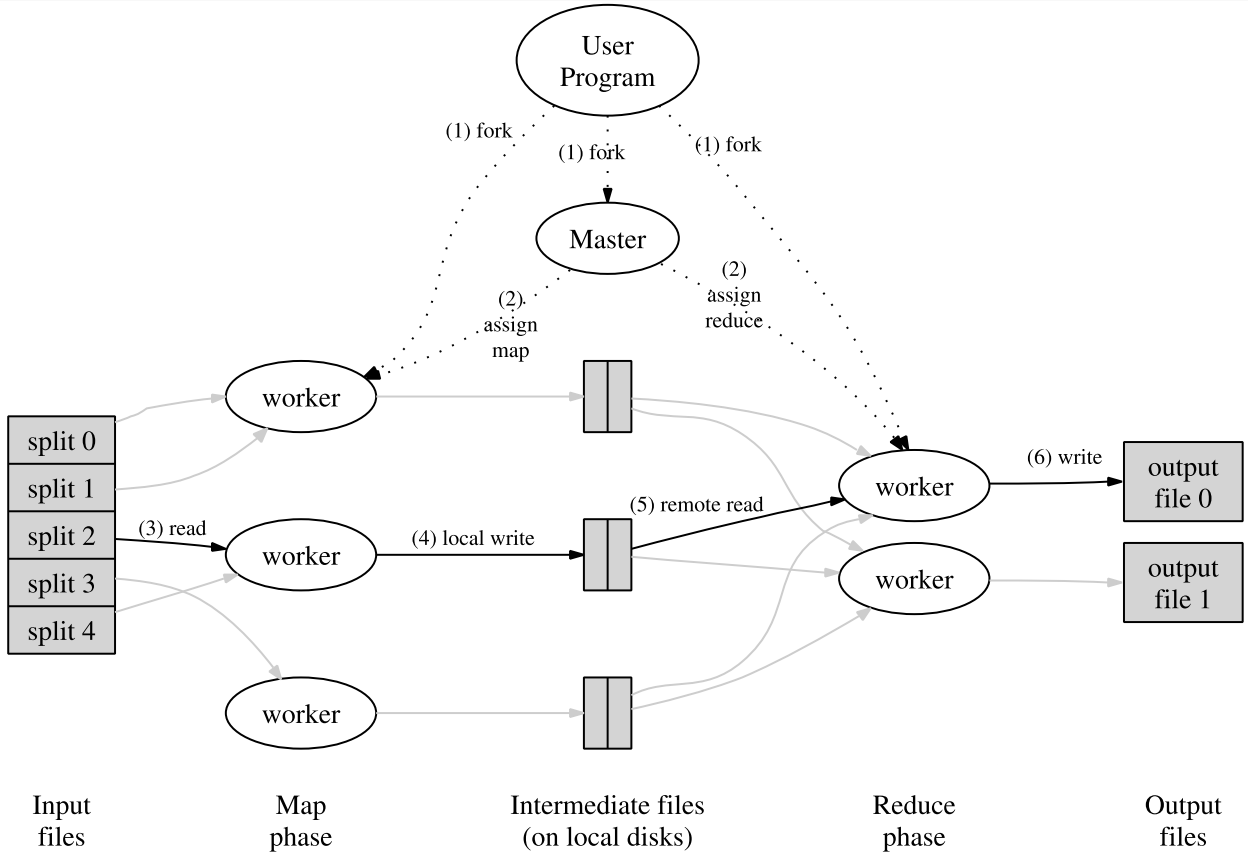
\includegraphics[width=\textwidth]{Abbildungen/mapreduce.png}
\caption[Übersicht der Ausführung von Googles MapReduce]{Übersicht der Ausführung von Googles MapReduce, Quelle: \cite{paper:mapreduce} S. 3}
\label{fig:mapreduce}
\end{figure}
Hadoop besitzt eine Master-Slave Architektur, wobei der Name-Node\footnote{damit ist der Master-Knoten gemeint, auch Jobtracker genannt} ankommende Anfragen bearbeitet und die Slave-Knoten organisiert.
Hadoop ist per API verwendbar und bietet sich somit zur Stapelverarbeitung an. %Todo: belegen
Es wird meist nur als Grundgerüst verwendet und mit Datenbanken wie HBase, MongoDB oder PostgreSQL sowie mit Frameworks für die Nutzung wie Hive, \Gls{pig}, \Gls{spark} oder Scalding erweitert.\\
%
Gegenüber der Möglichkeit auf unterschiedlicher Hardware direkt und gleichzeitig mit Terrabyte großen Daten zu arbeiten, steht die Kritik das MapReduce eine hohe IO auf Festplatten der einzelnen Systeme erzeugt, da alle Zwischenergebnisse auf den Festplatten abgelegt und anschließend gelesen werden.

\subsection{ZooKeeper}
\label{zookeeper}
Das Apache Projekt ermöglicht verteilten Prozessen über ZNodes miteinander zu kommunizieren.
ZNodes sind Datenhalter, welche ihre Daten in einem Namensraum versionieren.
Es wird häufig gleichzeit mit Hadoop\footnote{siehe \ref{hadoop}} eingesetzt.
Ziel ist dabei ein hoher Durchsatz, geringe Latenzen, Hochverfügbarkeit und effektiver Zugriff durch die Prozesse.
Dabei verwaltet ZooKeeper eine geringe Datenmenge von einigen Kilobyte, da einzig Metainformationen von Interesse sind.\footnote{siehe \cite{website:zookeeper}} 



\subsection{Thrift}
\label{thrift}
Thrift ist nach \cite{website:thrift} ein Framework zur Entwicklung skalierender Programmiersprachen übergreifender Dienste.
Es verbindet einen Softwarestapel mit einer generativen Engine.
Unterstützte Programmiersprachen sind C++, Java, Python, PHP, Ruby, Erlang, Perl, Haskell, C\#, Cocoa, JavaScript, Node.js, Smalltalk, OCaml, Delphi und andere.
Dabei muss sich der Entwickler nicht mit den einzelnen Schichten des OSI Modells beschäftigen und auch keine Eigenheiten der Programmiersprachen berücksichtigen.
Es werden Datentypen, der Transport mit Thrift eigenen Protokollen, die Datenversionierung und Gegenstellen der Dienste durch das Thrift Framework bereitgestellt.
Thrift wurde 2007 von Facebook freigegeben. \cite[S.1]{paper:thrift}


\subsection{Accumulo}
\label{accumulo}
%https://en.wikipedia.org/wiki/Apache_Accumulo
Hierbei handelt es sich um ein Apache Projekt, es ist eine Java Open-Source Implementation des BigTable Ansatzes von Google und wird seit 2008 entwickelt.
Es verwendet Hadoop, ZooKeeper und Thift.
Der BigTable Ansatz wird um Iteratoren, Zellenbezeichnungen, Constraints, physische Verteilungsmöglichkeiten einer dokumentbasierten Datenbank und die Unterstützung der gleichzeitigen Verwendung mehrerer HDFS namenodes erweitert.
Weitere Funktionen sind folgende:
\begin{itemize}
\item Verwendung mehrerer Master
\item Verwendung einer eigenen Zeitsynchronisation
\item Eingebaute temporäre Datenhaltung im Arbeitsspeicher
\item Bereitstellung von Testimplementierungen per API
\end {itemize}
Es existieren weiterhin verschiedene Erweiterungen zum Datenmanagement und Änderung des Ordnungsrahmens zur Verfügung. \cite{website:accumulo_features}

\subsection{GIS GeoMesa}

GeoMesa ist eine unter Apache License Version 2.0 stehende geografische Datenbank der Firma LocationTech\footnote{\url{https://www.locationtech.org/}} mit den Möglichkeiten der verteilten Verarbeitung und Versionierung von geografischen Daten.
Dieses Framework ist in \Gls{scala} geschrieben.
Es erweitert Accumulo\footnote{siehe \ref{accumulo}}, unterstützt die GeoTools API und bietet ein Plugin für den Mapserver \Gls{geoserver} an.
Die Daten werden nach Geohash %\footnote{siehe \ref{geohash}}
verwaltet. (vgl. \cite{website:geomesaeclipse})\\
GeoMesa wird in Verbindung mit stream processing\footnote{bspw. Spark oder Storm} und batch processing\footnote{bspw. Pig oder Cascading} verwendet.
Zur räumlichen Datenverarbeitung werden Scala Bibliotheken wie \Gls{jts} und GeoTools eingesetzt.
Vorrangig werden Vektordaten von GeoMesa verarbeitet, durch eine optionale Erweiterung sind auch Rasterdaten verwendbar.
Datenimport wird ingest genannt, erfolgt über die Kommandazeile und unterstützt die Datenformate CSV, TSV und SHP.
CSV, TSV, Shapefile, GeoJSON, and GML können dagegen über den selben Weg exportiert werden.
Weiterhin erfolgt der Datenexport und -import über Scala.
GeoMesa ist gedacht, um initial große Datenmengen per Ingest zu laden und diese anschließend mit Frameworks zur verteilten Datenverarbeitung wie Spark und dafür vorgesehenen Bibliotheken zu verarbeiten.
%\url{https://www.locationtech.org/proposals/geomesa} :\\
%- outperforming postgis with geoserver
%
%
%\url{http://de.slideshare.net/CCRinc/location-techdc-talk2-28465214}
%- Verwendung fraktaler Kurven
%- mit Spark und Scalding wesentlich schneller als PostGIS
%
%
%\url{https://docs.google.com/presentation/d/1NO0ppk8MfDs8Q-QcUidZCSZK7YYwd9RjJoHV1V4Yq_w/edit?pli=1#slide=id.p} :\\

%storm vs spark: http://xinhstechblog.blogspot.de/2014/06/storm-vs-spark-streaming-side-by-side.html https://stackoverflow.com/questions/24119897/apache-spark-vs-apache-storm http://www.zdatainc.com/2014/09/apache-storm-apache-spark/



%\subsection{Neo4J}

\subsection{Postgres-XL}
\label{grundlagen:postgresxl}
Postgres-XL ist ein frei verfügbares Clustersystem für PostgreSQL unter der Mozilla Public License.
XL steht dabei für eXtensible Lattice, erweiterbarer Verbund.
Damit soll es ermöglicht werden, mit PostgreSQL verteilt Schreiboperationen zu skalieren sowie parallele Datenverarbeitung auf mehreren physischen und virtuellen Systemen gleichzeitig zu betreiben.
Es handelt sich um ein shared nothing Mehrrechner-Datenbanksystem.
Dafür wird zur verteilten Datenhaltung \Gls{acid} mit \Gls{mvcc} und zur parallelen Verarbeitung ein \Gls{mpp} Mechanismus eingesetzt. (siehe \cite{website:postgresxl-about})
Die Postgres-XL Umgebung nutzt mehrere PostgreSQL Instanzen und bietet Schnittstellen für alle Instanzen an.\\
Abbildung \ref{fig:postgresxl} verbildlicht den Aufbau.
Laut Abbildung wird als erstes ein Load-Balancer angesprochen und es existieren mehrere GTM Instanzen.
Dies wird in der Dokumentation nicht belegt.
Die Elemente sind nach \cite{website:postgresxl-about} wie folgt beschrieben:
\begin{description}
\item[Global Transaction Manager] Dient als Verwaltungselement der Transaktionen und realisiert \Gls{mvcc} über das System. Laut Dokumentation existiert genau ein GTM pro Cluster, um \Gls{mvcc}  mit einem globalen Kontext realisieren zu können. Der GTM wird von jeder Coordinator Instanz angesprochen. Es wird jedoch zusätzlich pro physischem Knoten des Clusters ein GTM-Proxy empfohlen, welcher die Anfragen an den GTM bündelt.
\item[Coordinator] Jeder Coordinator dient als Eintrittspunkt in den Cluster, ruft von der GTM Instanz pro SQL Statement eindeutige Transaktionsnummern und globale Informationen ab sowie formuliert Subquerys für die relevanten DataNodes entsprechend seines Query-Planers.
\item[Data Node] Diese Elemente sind PostgreSQL Instanzen, welche die konkreten Daten vorhalten und das Transaktionsmanagement an den GTM abgegeben haben. Die Datenbanken und Tabellen der DataNodes werden entweder per partition verteilt oder repliziert. Anfragen können von verschiedenen Coordinators gleichzeitig in unterschiedlichen Sitzungen erfolgen. Auf Grund der Kapselung besitzt jeder Data Node seinen eigenen Kontext zur Transaktion.
\end{description}
Dabei besitzt jeder Coordinator und jeder DataNode einen ConnectionPool, welcher die Verbindungen verwaltet.
Veränderungen des Datenbankschemas werden auf alle Coordinators und DataNodes propagiert.
Es besteht jedoch die Möglichkeit einzelne DataNodes aus Relationen des Schemas zu entfernen.
Damit handelt es sich bei Postgres-XL um ein förderiertes Datenbanksystem.
Es wird analog einer PostgreSQL Installation angesprochen.
Zur Erhöhung der Ausfallsicherheit, besteht die Möglichkeit, für jedes Element im Cluster eine dazugehörige inaktive Instanz zu erzeugen, welche bei Ausfall der eigentlichen Instanz für diese einspringt.
Jedes Element im Cluster ist einzeln zu konfigurieren, was zu $ n*3+1 $ verschiedenen Konfigurationen bei $n$ DataNodes führt.
Zur Vereinfachung der Erstellung und Verwaltung eines Clusters sind neben den von PostgreSQL gelieferten Kommandozeilentools weitere durch Postgres-XL gegeben.
Zur Erstellung und Verwaltung eines Clusters kann pgxc-ctl eingesetzt werden.
Damit kann mit einer Konfigurationsdatei ein Cluster definiert sowie erstellt werden oder das Cluster mit einem Befehl um Knoten ergänzt werden.
\begin{figure}[h!]
\centering
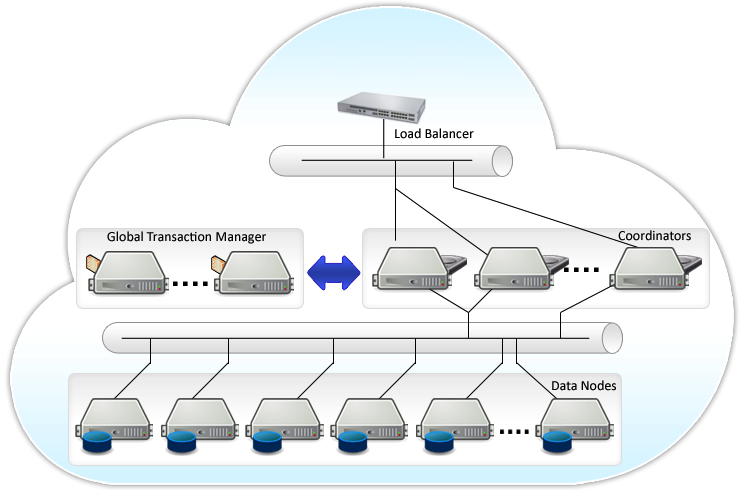
\includegraphics[width=.7\textwidth]{Abbildungen/postgresxl-structure.jpg}
\caption[Aufbau Postgres-XL]{Aufbau Postgres-XL, Quelle: \url{http://www.postgres-xl.org/wp-content/uploads/2014/04/xl_cluster_architecture1.jpg}}
\label{fig:postgresxl}
\end{figure}
%Das System wird somit analog einer PostgreSQL Instanz angesprochen.
Ebenso sind Erweiterungen wie PostGIS, DBLink oder PL/R installierbar.
Es ist zu erwähnen, dass die Version 9.2.34 keine Trigger unterstützt\footnote{siehe \url{http://files.postgres-xl.org/documentation/intro-whatis.html} Ergänzung 4} und und der Transition Typ internal nicht verwendet werden kann.
%Verteilung findet nach Attribut statt, schließt aber bigint aus
%Indexstrukturen nicht vergessen!
%replikationsverfahren wichtig?

\subsection{Array DBMS Rasdaman}

Rasdaman ist ein Array-Datenbanksystem speziell zum speichern und verarbeiten von Rasterdaten.
Es erweitert eine relationale Datenbank und wird mit  multi-dimensionalität der Daten, einer eigenen SQL ähnlichen Abfragesprache, Parallelisierung und Skalierbarkeit in beliebigen Maßstab sowie OGC konformen Diensten beworben.
Es ist als Client bzw. API unter der \Gls{lgpl} 3 und als Server unter der \Gls{gpl} 3 für Linux, MacOS und Solaris verfügbar.
Als OGC konforme Dienste werden WMS 1.3, WCS 2.0, WCS-T 1.4, WCPS 1.0 und WPS 1.0 bereitgestellt.
Die API kann in Java, C++ und über die eigene Abfragesprache rasql verwendet werden. (vgl. \cite{website:rasdamanogeo})
Der beschriebene Aufbau ist unter Abbildung \ref{fig:rasdaman} dargestellt.
\begin{figure}[h!]
\centering
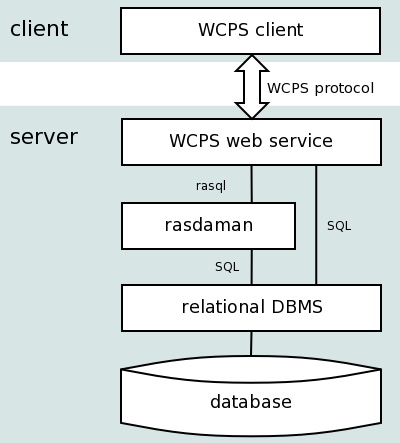
\includegraphics[width=.4\textwidth]{Abbildungen/rasdaman-aufbau.png}
\caption[Aufbau Rasdaman]{Aufbau Rasdaman, Quelle: \url{http://www.rasdaman.org/raw-attachment/wiki/Technology/wcps-stack.png}}
\label{fig:rasdaman}
\end{figure}

Es besteht die Möglichkeit, Rasdaman zu einer bestehenden PostgreSQL zu installieren und direkten Datenaustausch zwischen den beiden Systemen zu ermöglichen.
Weiterhin kann Rasdaman in Verbindung mit GDAL verwendet werden.
Momentan existiert eine Community und eine Enterprise Variante. Dabei verfügt die Enterprise Variante über mehr Features wie beispielsweise Datenkomprimierung, Serververwaltung per Webbrowser, Laufzeitoptimierungen und verschiedene Datenbankschnittstellen.
Von der verwendeten Datenbank wird BLOB als Datenbankinterner Datentyp verwendet. (vgl. \cite{website:rasdamanowiki})

\chapter{Ausgangsszenario}

\section{Anforderungen}
\label{Anforderungen}

% kartografisches Produkt
Aktuelle Möglichkeiten der Datenerfassung über Sensoren und moderne Probenahmegeräte führen zu mehr und mehr Datensätzen, die für einen Landwirtschaftsbetrieb ausgewertet werden müssen. Darüber hinaus besteht die Notwendigkeit, Daten Jahresübergreifend und betriebsübergreifend auszuwerten, um pflanzenbauliche Zusammenhänge über statistische Methoden untersuchen zu können.
In den letzten 3 Jahren wurde beispielsweise nur zum Thema N-Versorgung\footnote{Stickstoffdüngung und -aufnahme} für einen Betrieb etwa 800 Datensätze mit 1,9 Mio Einträgen erfasst. Alle diese Daten haben einen räumlichen Bezug, sie müssen weiterverarbeitet, kartographisch aufbereitet und dargestellt werden.\\
Daraus ergeben sich verschiedenen Anforderungen an die Technologie, die für die Verarbeitung, Analyse und Darstellung verwendet wird:
\begin{itemize}
\item PostgreSQL mit PostGIS zum Datenimport und -export nutzbar
\item Gruppieren und Filtern mit geringer Laufzeit
\item parallele Berechnung\footnote{hier Statistik bzw. Geostatistik sowie Interpolation} über große Datenmengen mit geringer Laufzeit
\item Räumliche Berechnungen wie Verschneiden, Berechnen von Overlays
\item  Unterschiedliche Prinzipien der Kartengenerierung, hier dynamisches rendern aus dem Datenbestand zur Laufzeit oder dynamisches rendern bei Dateneingang wodurch vorgerenderte Karten bereitstehen % caches wirklich mit untersuchen? wenn ja in Schnittstellen aufnehmen
\item nutzbare Schnittstelle zur Darstellung mit dem \Gls{umn}
\end{itemize}

% TODO: ergänzen, dass Anforderungne von Ist-Stand und möglichen Verbesserungen herrühren

% Eventuell technische SIcht extra darstellen, um Eignung der Systeme besser herausarbeiten zu können

Konkret handelt es sich bei den Eingangsdaten um folgende:
\begin{description}
\item[Pflanzenbauliche Daten]\footnote{Sensoren, Bodenuntersuchung, \Gls{bonitur}, Logger} Punktdaten
\item[Basisdaten wie Feldgrenzen] Vektordaten
\item[Externe Satelliteninformationen und Multispektralanalysen] Rasterdaten
\end{description}

\subsection{Softwarequalität}
\label{softwarequalität}
%TODO: warum hier die qualitätsmerkmale
Qualitätsmerkmale sind nach DIN 9126\footnote{DIN 9126 wurde durch ISO/IEC 25000 ersetzt, jedoch sind beide nur proprietär verfügbar} in \cite{book:lehrbuchsoftware} S. 258 f. Funktionalität, Zuverlässigkeit, Benutzbarkeit, Effizienz, Änderbarkeit und Übertragbarkeit.
Diese Merkmale werden durch Qualitätskriterien für jeden Anwendungsfall konkretisiert.


Nachfolgend werden die Qualitätsmerkmale für diesen Anwendungsfall konkretisiert und darauf die zu untersuchenden aufgelistet.


Da die zu analysierenden Systeme eine Datenbank beinhaltet, welche mit räumlichen Datentypen arbeitet, wurde die im Anhang C von \cite{book:objdbs} enthaltene Checkliste zur Auswahl eines \Gls{odbms} berücksichtigt.

\textbf{Funktionalität}\\
Das System stellt alle geforderten Funktionen mit den definierten Eigenschaften zur Verfügung.
\begin{description}
\item[Richtigkeit] Ergebnisse sind korrekt oder ausreichend genau. Die Ergebnisse sollen zu 99\% mit denen des Ist-Standes übereinstimmen.
\item[Interoperabilität] Es sind Schnittstellen zur Ein- und Ausgabe vorhanden. Dabei soll es sich um PostgreSQL Import sowie PostgreSQL und \Gls{umn} Export handeln.
\item[Funktionsumfang] Mindestens die benannte und essentielle Menge an Funktionalitäten wird bereitgestellt. Dazu zählt:
parallele Verarbeitung, Gruppierungs-, Filter-, Verschneidungs- sowie Overlayfunktionen, Geostatistik und Umrechnung zwischen Koordinatensystemen und -formaten. Außerdem sind vorhandene Datentypen und Schemaversionierung von Interesse.
\item[Ordnungsmäßigkeit] Die Implementation des Systems und dessen Funktionen erfüllt Normen, Vereinbarungen, gesetzliche Bestimmungen und andere Vorschriften. Hierzu ist zu nennen, dass besonders Berechnungsfunktionen nach mathematischen Gesetzen implementiert sein müssen. Konkret sind Berechnungen der räumlichen Verarbeitung nach anerkannten definierten Algorithmen durchzuführen.
\end{description}



\textbf{Zuverlässigkeit}
\begin{quote}
Fähigkeit einer Software, ihr Leistungsniveau unter festgelegten Bedingungen über einen festgelegten Zeitraum bewahren.\footnote{\cite{book:lehrbuchsoftware} S. 259}
\end{quote}
Nutzung von Tools zur Überwachung und Konfiguration immanent.
\begin{description}
\item[Fehlertoleranz] Das System sollte auftretende Fehler des Tagesgeschäftes abfangen und weiterarbeiten. Besonders Fehler in den Quelldaten können zu Fehlern während der Ausführung von Berechnungen führen, was per s\'{e} abgefangen werden muss.
\item[Wiederherstellbarkeit] Auch die Möglichkeit bei einem schwerwiegendem Fehler Daten und Stände der abgebrochenen Operationen wiederherzustellen ist ein zu betrachtendes Qualitätskriterium.
\item[\Gls{mttf}] Diese statische Kenngröße der erfahrungsgemäßen mittleren Lebensdauer ist für kritische Systeme relevant.
\end{description}



\textbf{Benutzbarkeit}\\
Qualität des Zugangs für Benutzer sowie Eignung für eine oder mehrere Benutzergruppen.
\begin{description}
\item[Verständlichkeit] 
\item[Bedienbarkeit] 
\item[Dokumentation] Eine ausführliche, aktuelle und korrekte Dokumentation ist Voraussetzung zur produktiven Verwendung.
\item[Eignung] Die angestrebte Benutzergruppe muss mit der aktuellen Benutzergruppe übereinstimmen. Die aktuelle Benutzergruppe ist Programmierer bzw. Administrator.
\end{description}



\textbf{Effizienz}\\
Das Verhältniss zwischen Auslastung der Hardware und erfolgreich bearbeiteten Aufgaben. Nach \cite{book:Leistungsanalyse} S. 21 ist Leistung paralleler Programme das Verhältnis des Speedups zur Anzahl der verwendeten Prozessoren. Wobei Speedup als Verhältnis der Ausführungszeiten zwischen der auf N Prozessoren ausgeführten parallelen Version eines Programms und der sequentiellen Version des Programmes definiert ist. Diese Definitionen treffen für die zu untersuchenden Systeme zu, da es sich um parallelisierende \Gls{gis} handelt.
\begin{description}
\item[Zeitverhalten] Oder auch Laufzeitverhalten genannt, dient allgemein zur Darstellung des Durchsatzes. Die Skalierung des Systems zählt hier dazu. Dies wird speziell durch zusätzliche Leistungstests beurteilt.
\item[Verbrauchsverhalten] Das Verhältnis aus erbrachter Leistung und dem dafür notwendig gewesenen Aufwand in Form von Hardwarenutzung.
\item[Skalierbarkeit] Anzahl der zu verwendenden Computer um nach dem Speedup eine Effizienzsteigerung im Gegensatz zum Einsatz bei einem Computer zu erreichen.
\end{description}



\textbf{Änderbarkeit}\\
Aufwand zur Verbesserung oder Anpassung der Umgebung und der Spezifikationen, auch Wartungsaufwand genannt.
\begin{description}
\item[Analysierbarkeit] \glqq Aufwand, um Mängel oder Ursachen von Versagen zu diagnostizieren oder um änderungsbedüftige Teile zu bestimmen.\grqq\ [\cite{book:lehrbuchsoftware} S. 260]
\item[Modifizierbarkeit] Notwendiger Aufwand für Änderungen zum Ziele der Verbesserung und Fehlerbehebung.
\item[Stabilität] Wahrscheinlichkeit vom ungewollten Auswirkungen von Änderungen.
\item[Prüfbarkeit] Oder Testbarkeit als Merkmal, welches die Möglichkeiten und den Aufwand zum testen der originalen und geänderten Systeme.
\end{description}



\textbf{Übertragbarkeit}\\
Die Fähigkeit das System auf andere Hard- und Software und andere Vorgehensweisen zu migrieren.
\begin{description}
\item[Anpassbarkeit] Möglichkeiten des unveränderten Systems Änderungen vorzunehmen.
\item[Installierbarkeit] Systemvoraussetzung und Aufwand zur Installation des Systems.
\end{description}



\textbf{nichttechnische Kriterien}\\
Erweiterte Qualitätskriterien, welche nicht nach der DIN 9126 zugeordnet werden können.
\begin{description}
\item[Herstellerfirma und Produkt] Dazu zählt die Marktposition, der Preis, die Produktplanung und Service.
\end{description}

Die zu untersuchenden Qualitätskriterien für die Softwareauswahl sind Funktionsumfang, Fehlertoleranz, Dokumentation, Zeitverhalten, Analysier- und Modifizierbarkeit.


\subsection{Qualitätsmetriken}
\label{qualitätsmetriken}
%TODO: essentielles markieren oder stärker wichten

\textbf{Richtigkeit:}\\
Berechnungen sind zu 99\% korrekt. Ausnahme ist dabei die Berechnung von Koordinaten. Dabei haben die Ergebnisse bis acht Stellen nach dem Komma korrekt zu sein.
Die statische Abbildung ist dabei $[korrekt, nicht\ korrekt]\ nach\ [1, 0]$.

\textbf{Interoperabilität:}\\
Import und Export von räumlichen Daten aus PostgreSQL sowie eine Anbindungsmöglichkeit an den \Gls{umn}.
Statische Abbildung:\\
$[Datenschnittstelle\ und\ UMN\ Schnittstelle\ vorhanden,Datenschnittstelle\ vorhanden,$\\$UMN\ Schnittstelle\ vorhanden,keine\ Schnittstelle\ vorhanden]\ nach\ [10,7,2,0]$\\
Der Bereich bis zehn soll die Wichtigkeit des Vorhandenseins der Schnittstellen verdeutlichen.

\textbf{Funktionsumfang:}\\
Folgende gibt die Wertung der Existenz der einzelnen Funktionen wieder.
Existiert die Funktion nicht, ist die Wertung Null.
\begin{table}[h]
\centering
\begin{tabular}{l|l}
\textbf{Funktion} & \textbf{Wertung} \\ \hline
parallele Verarbeitung & \psum{2} \\ \hline
geografische Datentypen & \psum{14} \\ \hline
Umrechnung zwischen Koordinatensystemen & \psum{10} \\ \hline
Gruppierungsfunktionen & \psum{10} \\ \hline
Verschneidungsfunktionen & \psum{4} \\ \hline
Overlayfunktionen & \psum{4} \\ \hline
Geostatistik & \psum{6} \\ \hline
Filterfunktionen & \psum{10} \\ \hline
Schemaversionierung & \psum{1}
\end{tabular}
\caption{Wertungstabelle Funktionsumfang}
\label{table:funktionsumfang}
\end{table}
Maximale Wertung: \FPtrunc\Gesamtsumme\Gesamtsumme{0}\FPprint\Gesamtsumme

\textbf{Fehlertoleranz:}\\
Es gilt zu messen, ob Fehler bei einer Berechnung andere verschränkt gleichzeitig laufende Berechnungen beeinträchtigt.
Aus diesem Grund wird Unabhängigkeit auf eins und Abhängigkeit auf null abgebildet.

\textbf{Dokumentation:}\\
Vorhandene Dokumentation ist nach einzelnen Themen zu bewerten.
Dabei kann ein maximaler Wert von 13 erreicht werden.
\begin{table}[h]
\centering
\begin{tabular}{l|l}
\textbf{Dokumentation zu} & \textbf{Wertung je Eintrag} \\ \hline
Installation, Zeitverhalten & 1 \\ \hline
Funktionsumfang & 2 \\ \hline
Interoperabilität, Best practise, Anpassbarkeit & 3 
\end{tabular}
\caption{Wertungstabelle Dokumentation}
\label{table:dokumentation}
\end{table}

\textbf{Zeitverhalten:}\\
%TODO: Werte aus Ist-Stand in Bezug auf Lasttests verwenden


\textbf{Modifizierbarkeit:}\\
Anpassungen des Frameworks hinsichtlich der folgenden Punkte erhöhen den Wert um eins:\\
Verwendung eigener Datentypen, Erstellung eigener Schnittstellen, Erstellung eigener Funktionen, Verwendung der Programmiersprachen Scala oder R, anlegen eigener Berechnungsvorgängen zur späteren Abarbeitung

\subsection{Testfälle}

%Qualitätskriterien auswählen und Metriken definieren - Usecases bzw, Funktionstests bzw. Testfälle definieren
%

\section{Ist-Stand}
\label{IstStand}
%groben Ablauf textuell und grafisch darstellen
% geplanten Einsatz des Prototypen ebenso darstellen 

\chapter{Systemauswahl}
\label{chapter:systemauswahl}
Mit den unter \ref{qualitätsmetriken} erstellten Metriken sind die Frameworks GeoMesa, Postgres-XL und Rasdaman zu vergleichen.
Der Vergleich findet im Rahmen einer Nutzwertanalyse statt.
Hierbei werden keine Daten von durchgeführten Tests herangezogen, sondern es wird anhand der Spezifikation der einzelnen Frameworks untersucht ergo eine Inspektion als Prüfmethode verwendet.

\section{Definition der Nutzwertanalyse}
\label{section:definitionnutzwertanalyse}
Die drei Frameworks wurden aus der Tabelle der Abbildung \ref{fig:spatialdatabases} ausgewählt.
\begin{figure}
\centering
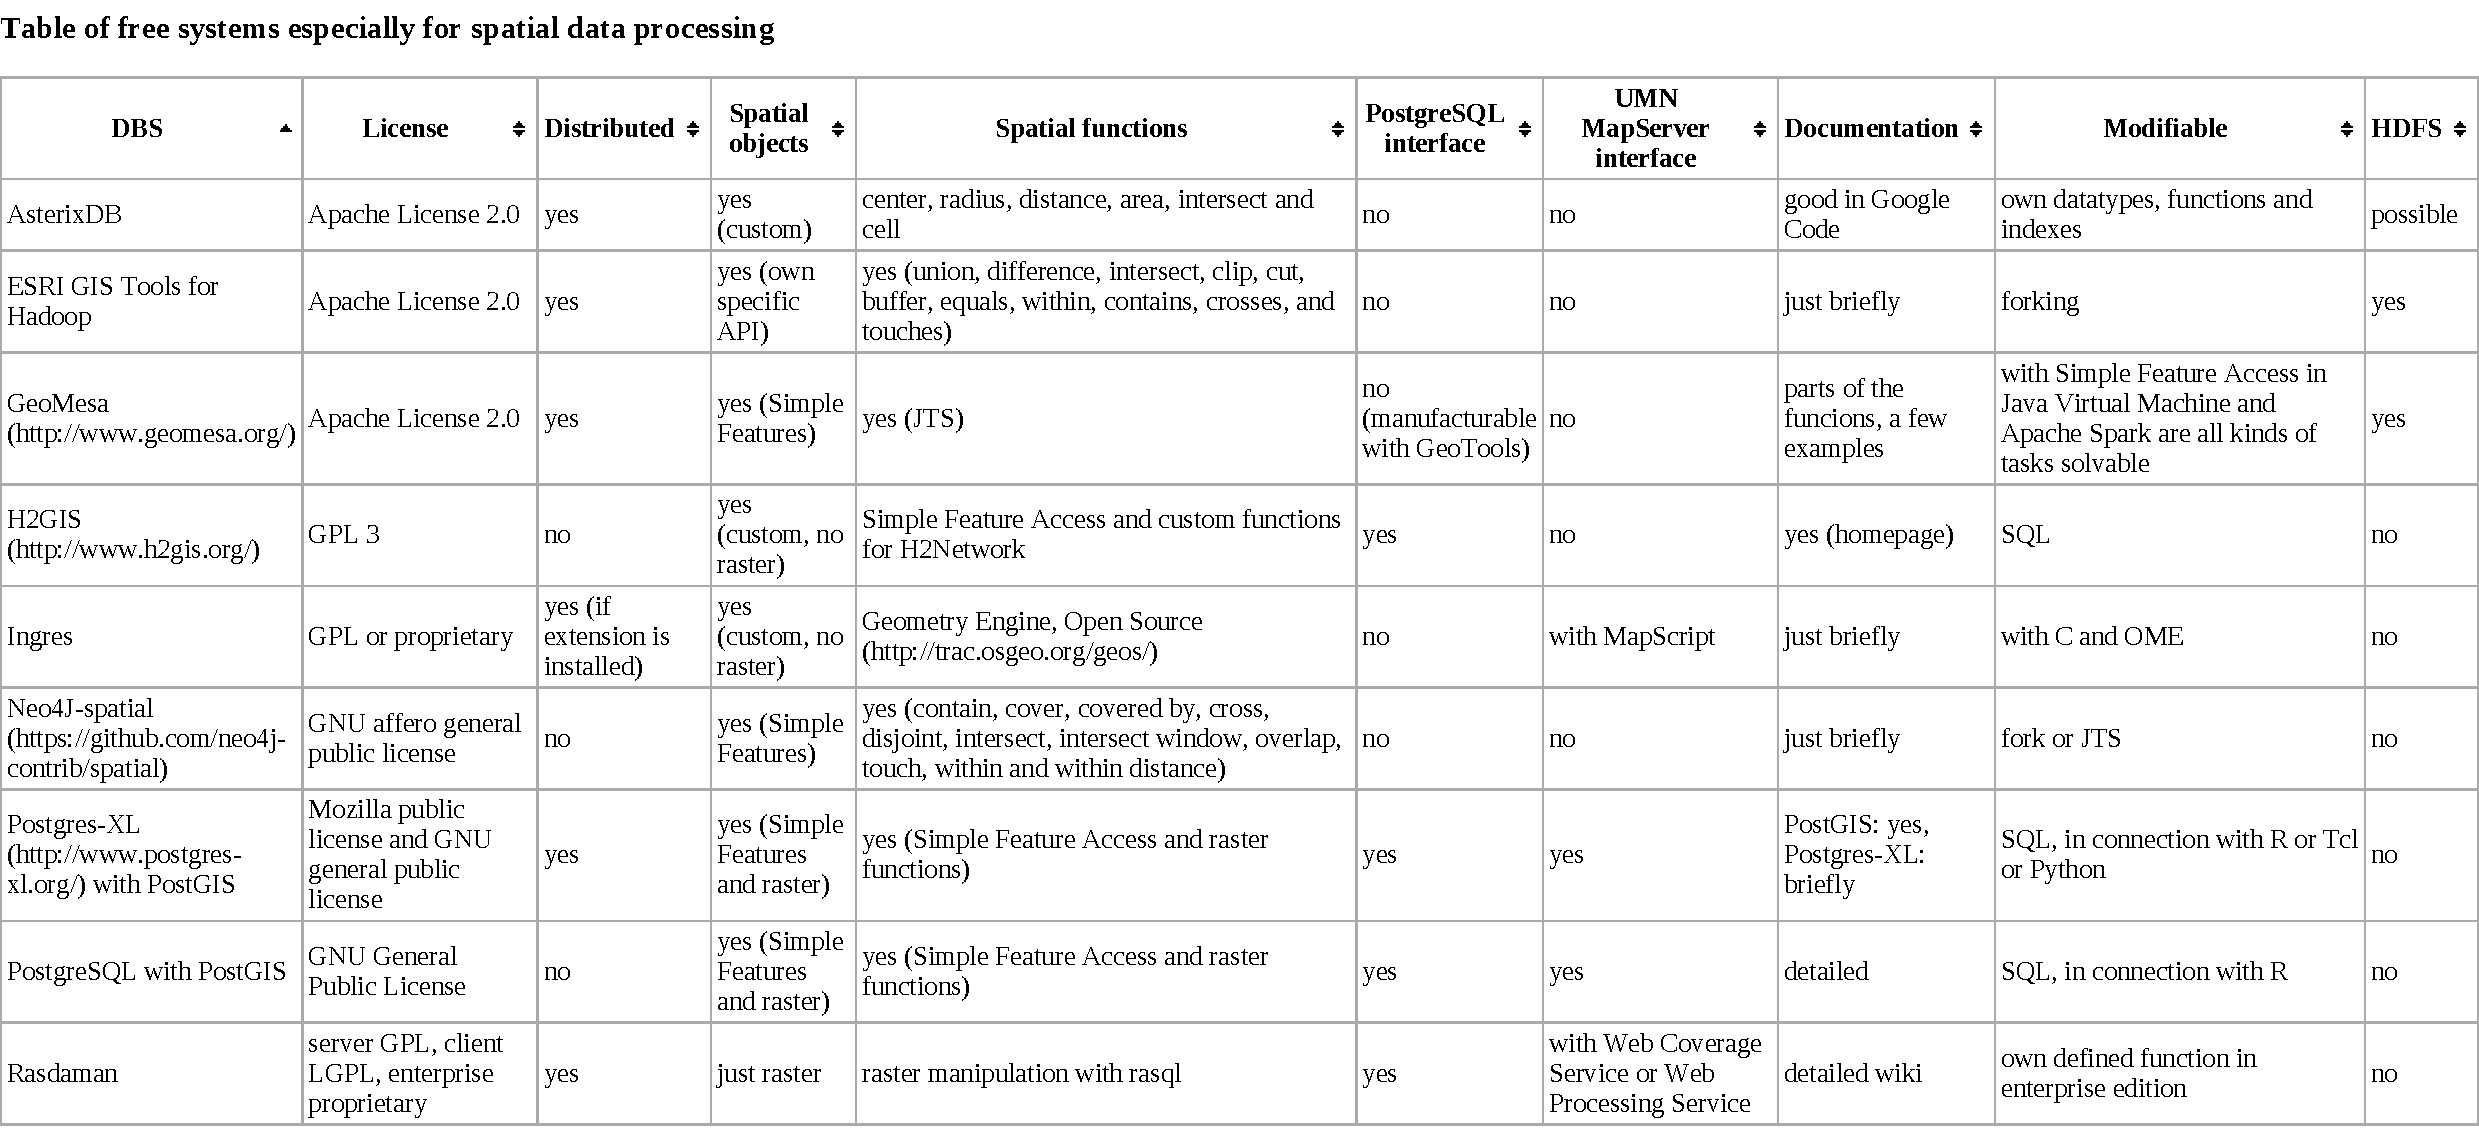
\includegraphics[angle=90,width=.66\textwidth]{Abbildungen/table_spatialdatabases_13_2_15.pdf}
\caption[Übersicht relevanter GIS Frameworks]{Übersicht relevanter GIS Frameworks nach \cite{website:wiki-spatialdatabase} vom 13.2.2015}
\label{fig:spatialdatabases}
\end{figure}
Darin sind GIS zur räumlichen Datenverarbeitung mit wesentlichen Eigenschaften wie \mbox{PostgreSQL} Schnittstelle und räumliche Datentypen aufgelistet.
Entsprechend den Anforderungen wurden daraus drei Frameworks für die Nutzwertanalyse ausgewählt.
Anforderung war dabei, dass Schnittstellen zu PostgreSQL und \Gls{umn} gegeben sind und es sich um ein Open-Source Frameworks handelt.

Abbildung \ref{fig:spatialdatabases} stammt von der Wikipedia Seite \url{https://en.wikipedia.org/wiki/Spatial_database} und ist für Unternehmen relevant, wie unter Kapitel \ref{aufrufe-spatialdatabases} beschrieben.
Der Autor erschuf die abgebildete Tabelle durch Recherche und stellte sie am 1.2.2015 in den Artikel.
In der Annahme, dass unternehmensbezogene Besucher der Seite fehlendes ergänzen oder falsches korrigieren würden, dient diese zur Auswahl geeigneter Frameworks.

Tabelle \ref{table:Wertungsmassstab} zeigt die für die Nutzwertanalyse notwendige Wertung der einzelnen Metriken.
Die Metriken Richtigkeit, Fehlertoleranz und Zeitverhalten werden nicht in die Analyse aufgenommen, da sie über die Spezifikation nicht belegbar sind.
\begin{table}[h!]
\centering
\begin{tabular}{|l|l|}
\hline
\textbf{Metrik} & \textbf{Gewichtung in \%} \\ \hline
%Richtigkeit & 10 \\ \hline
Interoperabilität & 30 \\ \hline
Funktionsumfang & 20 \\ \hline
%Fehlertoleranz & 8 \\ \hline
Dokumentation & 35 \\ \hline
%Zeitverhalten & 16 \\ \hline
Modifizierbarkeit & 15 \\ \hline
\end{tabular}
\caption{Wertungsmaßstab der einzelnen Metriken}
\label{table:Wertungsmassstab}
\end{table}
Für jedes Framework wird eine Nutzwertanalyse durchgeführt und die dazugehörige Tabellen dazu präsentiert.
Zu jeder Metrik wird der erreichte Wert, die ungewichtete Erfüllung, die gewichtete Erfüllung und ein Kommentar angegeben.
Die ungewichtete Erfüllung bezieht sich auf den maximal zu erreichenden Wert der Metrik, die gewichtete Erfüllung dagegen auf die Erfüllung der Metrik in Bezug auf Tabelle \ref{table:Wertungsmassstab}.
Die Kommentarspalte dient der Darstellung des Erreichens der Mindestanforderungen.
Der schlussendliche Nutzwert ergibt sich nach Zangemeister in \cite{website:nutzwertanalyse} aus der Summe der Produkte des Teilnutzens des jeweiligen Kriteriums mit der Gewichtung des Kriteriums.
Der Teilnutzen ist hier der Prozentuale Anteil der erreichten Punktzahl an der maximalen Punktzahl des Kriteriums.
Diese Prozentangabe wird als Wert mit der Gewichtung des Kriteriums multipliziert, woraus sich der Nutzwert für das Kriterium ergibt.
Die Summe aller dieser Teilnutzwerte ergibt den Nutzwert des Frameworks für den Anwendungsfall.

\section{Nutzwertanalyse}
Dieses Unterkapitel leg die Ergebnisse der Nutzwertanalysen zu den Frameworks GeoMesa, Postgres-XL und Rasdaman dar.
Die granulare Bewertung der einzelnen Kriterien der drei Systeme ist dagegen im Anhang \ref{appendix:systembewertung} zu finden.

\subsection{GeoMesa}
\begin{table}[h!]
\centering
\small
\begin{tabular}{|l|p{1.8cm}|l|p{3.1cm}|p{1.8cm}|}
\hline
\textbf{Metrik} & \textbf{erreichter Wert} & \textbf{Erfüllung in \%} & \textbf{Kommentar} & \textbf{gewichteter Teilnutzen} \\ \hline
Interoperabilität & 7 & 58 & Implementationen für beide Schnittstellen notwendig. & 17 \\ \hline
Funktionsumfang & 48 & 79 & Die meisten Funktionen sind nur mit Scala verfügbar, Mindestabdeckung jedoch gegeben. & 16 \\ \hline
Dokumentation & 4 & 31 & Mindestabdeckung nicht erfüllt. & 11 \\ \hline
Modifizierbarkeit & 4 & 80 & Mit Simple Features und Spark umfangreiche Problemlösungen erstellbar. Fehlende Funktionen können nachgerüstet werden. & 12 \\ \hline
\end{tabular}
\caption{Nutzwertanalyse GeoMesa}
\label{table:nutzwertanalyse-geomesa}
\end{table}
Der Nutzwert von GeoMesa ist nach Tabelle \ref{table:nutzwertanalyse-geomesa} 56.
Die detaillierte Analyse und Bewertung ist im Anhang \ref{appendix:systembewertung-geomesa} zu finden.
Darin waren die wichtigsten Quellen die offiziellen Webseiten von GeoMesa \cite{website:geomesa-tutorials} und \cite{website:geomesa-simplefeatures} sowie der Artikel \cite{website:geomesaeclipse}.

Neben dem messbaren Nutzwert sind die nichttechnischen Kriterien zu nennen, welche auf die Auswahl eines Frameworks Einfluss haben.
Dazu zählt die Herstellerfirma mit Marktposition, Produktplanung und Service sowie das Produkt in Hinsicht auf Preis, Lebendigkeit in Form von Entwickleraktivität und Größe der Benutzer.\\
\url{https://github.com/locationtech/geomesa} zählt am 17.2.2015 271 commits, 20 contributors und 186 branches.
Eine solche hohe Anzahl an branches spricht normalerweise für eine hohe Nutzung und Lebendigkeit des Projektes.
Jedoch wurde die Mehrzahl der branches nicht in den master Zweig übernommen.
\begin{figure}[h!]
\centering
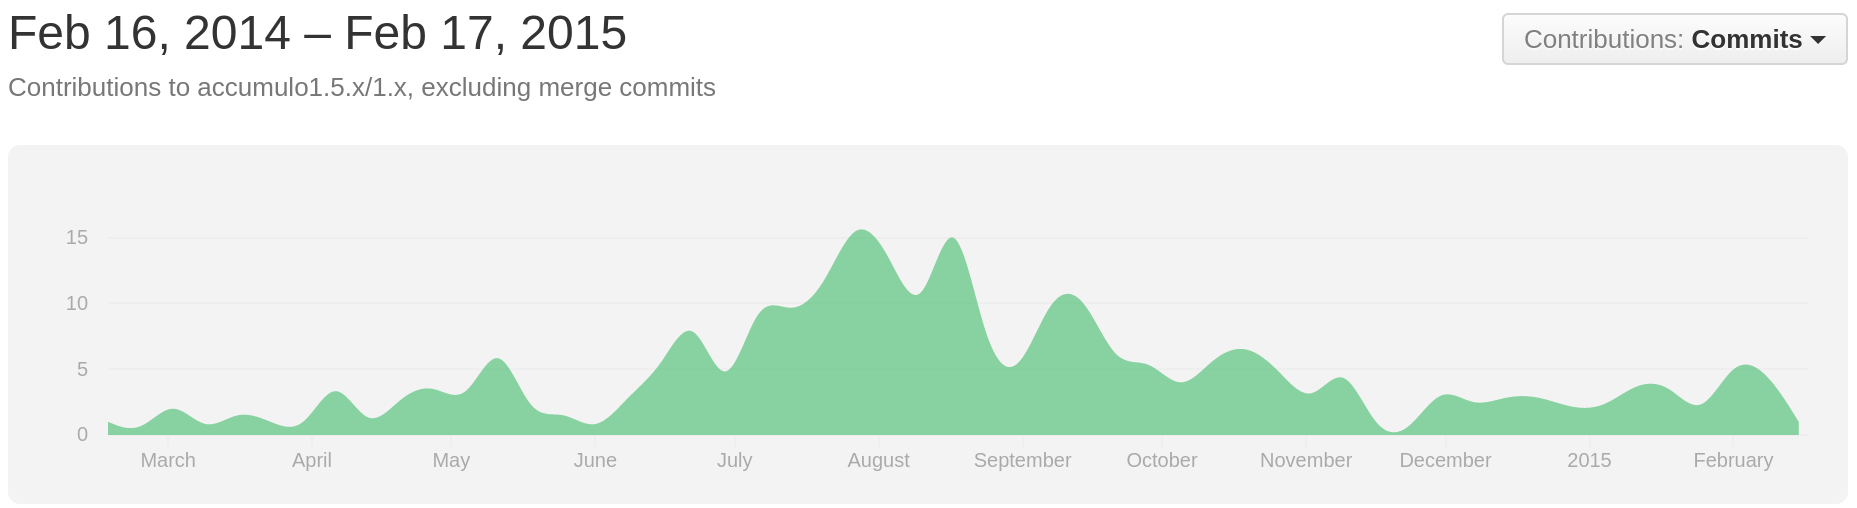
\includegraphics[width=\textwidth]{Abbildungen/geomesa_timeline_contributors.png}
\caption[Zeitleiste der contributor von GeoMesa]{Zeitleiste der contributor von GeoMesa vom 17.2.2015 nach \url{https://github.com/locationtech/geomesa/graphs/contributors}}
\label{fig:timeline_contr_geomesa}
\end{figure}
\begin{figure}[h!]
\centering
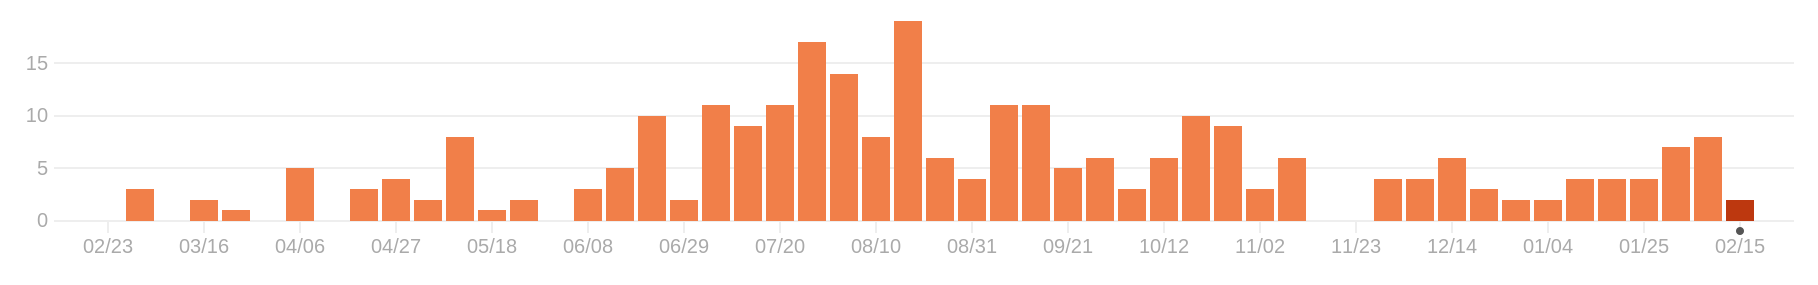
\includegraphics[width=\textwidth]{Abbildungen/geomesa_timeline_commits.png}
\caption[Zeitleiste der commits von GeoMesa]{Zeitleiste der commits von GeoMesa vom 17.2.2015 nach \url{https://github.com/locationtech/geomesa/graphs/commit-activity}}
\label{fig:timeline_commits_geomesa}
\end{figure}
Das GeoMesa Projekt auf GitHub hat nach Abbildung \ref{fig:timeline_contr_geomesa} eins bis vier Stammprogrammierer und ist im zweiten und dritten Quartal gegenüber mit der doppelten Anzahl an contributors gegenüber den anderen Quartalen fragmentiert.
Die drei contributors mit dem größten Anteil an Änderungen sind vorwiegend in Projekten von LocationTech aktiv was darauf schließen lässt, dass sie für das Unternehmen arbeiten.
Daraus folgt das zum wesentlichen Teil das Unternehmen LocationTech das Projekt wartet.
Die Anzahl der commits geht mit dem Verlauf der aktiven Programmierer einher.
Abbildung \ref{fig:timeline_commits_geomesa} zeigt die selbe Quartalsweise Verteilung wie Abbildung \ref{fig:timeline_contr_geomesa}.
Dabei ist der Unterschied zwei zu neun commits pro Woche.

LocationTech ist eine Arbeitsgruppe der non-for-profit Stiftung Eclipse.
In diesem Rahmen erhält diese Arbeitsgruppe 20 Mitglieder für Projektplanung und Projektumsetzung.
Weiterhin findet die Finanzierung im Rahmen von Mitgliedschaft an der Arbeitsgruppe statt.
Darin können Mitglieder je nach Beitrag Teile der Entscheidungsorgane der Arbeitsgruppe werden und Zugang zu Ergebnissen dieser erhalten. \cite{website:locationtech-about}
LocationTech ist mit GeoMesa mitten in der Entwicklung und hat keine durchgängig aktive Unterstützer.
Dieser Stand spricht gegen eine Auswahl von GeoMesa zum produktiven Einsatz.

\subsection{Postgres-XL}
\label{gegenuerbestellung:postgresxl}
\begin{table}[h!]
\centering
\small
\begin{tabular}{|l|p{1.8cm}|l|p{3.1cm}|p{1.8cm}|}
\hline
\textbf{Metrik} & \textbf{erreichter Wert} & \textbf{Erfüllung in \%} & \textbf{Kommentar} & \textbf{gewichteter Teilnutzen} \\ \hline
Interoperabilität & 12 & 100 & Analog des Ist-Standes. & 30 \\ \hline
Funktionsumfang & 53 & 87 & Mindestabdeckung erfüllt, jedoch sind Geostatistik und Versionierung nicht vorhanden. & 17 \\ \hline
Dokumentation & 9 & 69 & Dokumentation zu PostGIS ist sehr gut, zu Postgres-XL grob. Mindestabdeckung ist erfüllt. & 24 \\ \hline
Modifizierbarkeit & 5 & 100 & Vollständige Abdeckung vorhanden. Möglichkeiten sind in SQL gegeben. & 15 \\ \hline
\end{tabular}
\caption{Nutzwertanalyse Postgres-XL}
\label{table:nutzwertanalyse-postgresxl}
\end{table}
Aus Tabelle \ref{table:nutzwertanalyse-postgresxl} ergibt sich ein Nutzwert von 86.
Das Ergebnis bezieht sich auf Anhang \ref{gegenuerbestellung:postgresxl}.
Es wurde vorrangig die Postgres-XL Dokumentation \cite{website:postgresxl-manual} und jene von PostGIS \cite{website:postgisdocu-functions} verwendet.

Dazu sind ebenso nichttechnische Faktoren zu berücksichtigen.\\
\url{https://github.com/snaga/postgres-xl} zählt am 17.2.2015 35.266 commits, 23 contributors und drei branches.
\begin{figure}[h!]
\centering
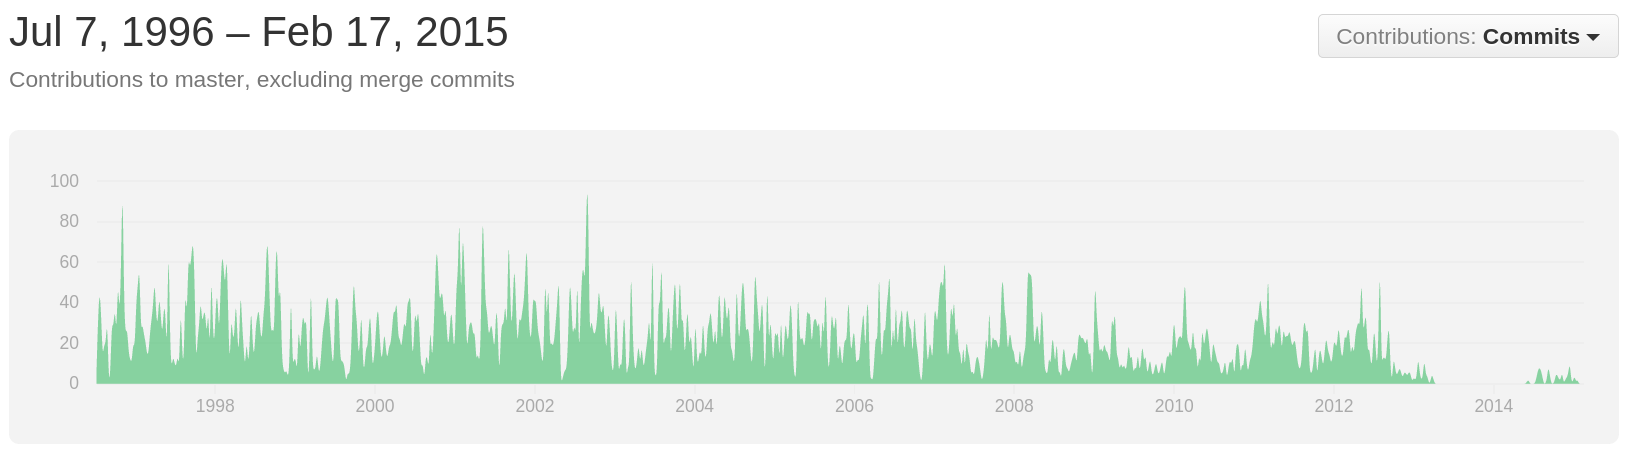
\includegraphics[width=\textwidth]{Abbildungen/postgresxl_timeline_contributors.png}
\caption[Zeitleiste der contributor von Postgres-XL]{Zeitleiste der contributor von Postgres-XL vom 17.2.2015 nach \url{https://github.com/snaga/postgres-xl/graphs/contributors}}
\label{fig:timeline_contr_postgresxl}
\end{figure}
\begin{figure}[h!]
\centering
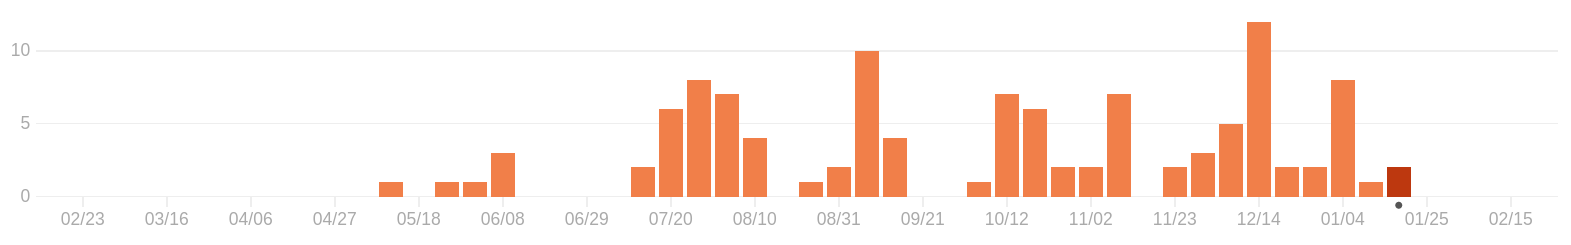
\includegraphics[width=\textwidth]{Abbildungen/postgresxl_timeline_commits.png}
\caption[Zeitleiste der commits von Postgres-XL]{Zeitleiste der commits von Postgres-XL vom 17.2.2015 nach \url{https://github.com/snaga/postgres-xl/graphs/commit-activity}}
\label{fig:timeline_commits_postgresxl}
\end{figure}
Abbildung \ref{fig:timeline_contr_postgresxl} zeigt einerseits, dass dieses Projekt seit 1998 besteht, andererseits das die Zahl der aktiven contributors im Gegensatz der Jahre 1998 bis 2012 zu 2014/2015 in etwa ein viertel beträgt.
Diese deutliche abrupte Abnahme der aktiven Programmierer deutet eine Veränderung im Projekt oder den Projektverantwortlichen an.
Die commits des vergangenen Jahres sind in Abbildung \ref{fig:timeline_commits_postgresxl} dargestellt.
Danach wurden im ersten Halbjahr 2014 nur insgesamt 6 commits und im zweiten Halbjahr 2014 etwa täglich ein commit durchgeführt.

Das Unternehmen TransLattice\footnote{\url{http://www.translattice.com/}} übernahm im Mai 2014 das Unternehmen StormDB.
Die Übernahme schloss das Projekt Postgres bzw. Postgres-XC ein. (siehe \cite{website:translattice-stormdb})
Dieses wurde darauf in Postgres-XL umbenannt und erweitert.
Diese Änderung rief die Verringerung der contributors seit Anfang 2014 hervor.
TransLattice verwaltet seitdem das Projekt und stellt technischen sowie theoretischen Support.
Postgres-XL ist durch die langjährige Entwicklung empfehlenswert für den produktiven Einsatz.
Jedoch ist die Aktivität der TransLattice Entwickler zu beobachten, da die Gefahr besteht, dass dieses Projekt vom Unternehmen nicht mehr gefördert wird und somit Fehler und Verbesserungen nicht eingepflegt werden und neue PostgreSQL Versionen nicht unterstützt werden.


\subsection{Rasdaman}
\begin{table}[h!]
\centering
\small
\begin{tabular}{|l|p{1.8cm}|l|p{3.1cm}|p{1.8cm}|}
\hline
\textbf{Metrik} & \textbf{erreichter Wert} & \textbf{Erfüllung in \%} & \textbf{Kommentar} & \textbf{gewichteter Teilnutzen} \\ \hline
Interoperabilität & 7 & 58 & \Gls{umn} Schnittstelle ist nicht vorhanden. & 17 \\ \hline
Funktionsumfang & 10 & 16 & Umfangreiche Rasterverarbeitung möglich. Kostenlose Version enthält keine Optimierungen. Abbildung von Simple Features auf Arrays mit Aufwand verbunden und nur bedingt sinnvoll. Mindestabdeckung wird nicht erfüllt. & 3 \\ \hline
Dokumentation & 8 & 62 & Mindestabdeckung erfüllt. & 22 \\ \hline
Modifizierbarkeit & 3 & 60 & Einfache Java und C++ API bietet zwar Erweiterungsmöglichkeiten, aber die Mindestabdeckung ist durch fehlende Datentypen nicht gegeben. & 9 \\ \hline
\end{tabular}
\caption{Nutzwertanalyse Rasdaman}
\label{table:nutzwertanalyse-rasdaman}
\end{table}
Aus Tabelle \ref{table:nutzwertanalyse-rasdaman} ergibt sich ein Nutzwert von 51.
Die granulare Bewertung befindet sich im Anhang \ref{appendix:systembewertung-rasdaman}.
Als Quelle diente dabei \cite{website:rasdaman-features} mit verlinkten Websites des gleichem Domain Namen.

Die Statistiken der Entwicklung des Repository müssen händisch gewonnen werden, da es auf einem Trac Verwaltungssystem mit Git basiert.
Das Repository ist unter\\\url{kahlua.eecs.jacobs-university.de/rasdaman.git} verfügbar.
Es kann mit der Konsolenanwendung Git heruntergeladen und ausgewertet werden.
So erhält man mit \textit{git log --pretty=format:\grqq \%h - \%an, \%ad : \%s\grqq\ | tail -1} das der erste commit 2009 erstellt wurde:
\begin{quote}
0f1055b - Constantin Jucovschi, Tue Mar 31 06:18:54 2009 -0400 : Initial commit
\end{quote}
Somit sind auch die commits des vergangenen Jahres ermittelbar.
So wurden vom 19.2.2014 bis zum 19.2.2015 1949 commits durchgeführt.
\textit{git shortlog -sne} liefert dagegen alle Autoren der vorhandenen commits.
Die Autoren der meisten commits sind Dimitar Misev mit 456, Piero Campalani mit 301 und Andrei Aiordachioaie mit 74 commits, Stand 19.2.2015 14:00 Uhr.
Herr Misev ist %laut seinem Linkedin Profil auf\\\url{https://de.linkedin.com/in/dimitarmisev}
Director of Product Development der \mbox{rasdaman} GmbH.
Herr Campalani und Herr Aiordachioaie haben wie Herr Misev an der Jacobs Universität in Bremen studiert, arbeiten aber nicht bei der \mbox{rasdaman} GmbH.

Rasdaman ist laut der Meldung \glqq Führender Rasterserver kostenfrei zum Download\grqq\ in \cite{website:rasdaman-newsarchive} seit September 2008 in einer freien Version verfügbar.
Außerdem ist es aus Forschungsarbeiten der TU Darmstadt, der TU München und der Jacobs Universität Bremen entstanden.
Förderer war dabei Community Research and Development Information Service der EU. \cite{website:rasdaman-cordis}

\section{Zusammenfassung}
%Auf Hypothese zu sprechen kommen - durch hinreichenden Informationsgehalt und empirische Beobachtungen bewiesen
Auf Grund der Ähnlichkeit von Postres-XL zum Ist-Stand erfüllt es nicht nur alle Mindestanforderungen, sondern erzielt auch den höchsten Nutzwert der untersuchten Frameworks.
Der Nutzwert von 86 ist auf 86\% Erfüllung der untersuchten Qualitätsmetriken abbildbar.
Da die Anforderungen neben vorhandenen Qualitäten des Ist-Standes fehlende dessen enthalten, betont diese hohe Erfüllung die Eignung für zukünftige Anforderungen an Zeitverhalten und Modifizierbarkeit.
Weiterhin spricht die Existenz seit 1996 für Postgres-XL.
Einzig die Übernahme der Firma TransLattice und der damit einhergegangene Einbruch der Anzahl an commits und contributors ist negativ und für die Zukunft zu beobachten.

GeoMesa und Rasdaman sind für andere spezielle Anwendungsfälle geeignet.
So ist Rasdaman in der kommerziellen Version bei verteilter Rasterdatenverarbeitung zu empfehlen.
GeoMesa eignet sich auf Grund des BigTable Ansatzes für enorm große Datenmengen die im Peta Bereich liegen.
So können diese Daten nicht nur gespeichert, sondern auch mit Scala und dazugehörigen Frameworks und Bibliotheken verteilt und parallel nach selbst erstellten Algorithmen und Vorgängen verarbeitet werden.

Die Systemauswahl hat nicht nur ein geeignetes Framework als Ergebnis, sondern auch ein Grundgerüst zur Beurteilung anderer Frameworks und Anwendungsfälle anhand von Nutzwertanalysen.
In Folge ist Postgres-XL detailliert zu untersuchen und erneut zu bewerten.

\chapter{Fazit}
%4-5 Seiten
In diesem letzten Kapitel wird das ausgewählte Framework Postgres-XL erneut einer Nutzwertanalyse unterzogen, da die vorhergehenden Kapitel neue Erkenntnisse hervorbrachten.
Im Anschluss wird diese Arbeit zusammengefasst und die Ergebnisse dieser mit Schwerpunkt der Nutzwertanalyse für Agri~Con gewertet.
Diese Arbeit und dieses Kapitel enden mit einem Abschnitt zum Ausblick, in welchem die zukünftige Nutzung der gewonnenen Erkenntnisse allgemein und bei Agri~Con erläutert wird.

\section{Nutzwertanalyse}
Aufbauend auf die Definition der Nutzwertanalyse in Abschnitt \ref{section:definitionnutzwertanalyse} wird diese erweitert, um die Ergebnisse aus den Tests in Kapitel \ref{chapter:tests} zu berücksichtigen.

%Wertungsmaßstab ergänzen und anpassen
\begin{table}[h!]
\centering
\begin{tabular}{l|l}
\textbf{Metrik} & \textbf{Gewichtung in \%} \\ \hline
Interoperabilität & 20 \\ \hline
Funktionsumfang & 20 \\ \hline
Dokumentation & 15 \\ \hline
Zeitverhalten & 40 \\ \hline
Modifizierbarkeit & 5
\end{tabular}
\caption{Neuer Wertungsmaßstab der einzelnen Metriken}
\label{table:Wertungsmassstab2}
\end{table}
Nach Erfassung der Testergebnisse der Leistung, wird in diesem Schritt das Zeitverhalten zusätzlich in einer erneuten Nutzwertanalyse bewertet.

Die Interoperabilität wird weiterhin mit zwölf Punkten bzw. 100\%{} Erfüllung bewertet, da die Ergebnisse der Funktionstests beweisen, dass beide Schnittstellen verwendet werden können.

Die Erkenntnisse, welche durch die Durchführung der Funktions- und Leistungstests entstanden sind, bedingen eine Änderung der Punkte für den Funktionsumfang.
Verschneidungsfunktionen sind wie in FT05 gezeigt vorhanden und einsetzbar, weshalb der Wert dafür auf vier erhöht wird.
Vermindert wird dagegen der Wert der Parallelität auf eins, da Funktionen des Lasttestes der Verarbeitung nicht gleichzeitig genutzt werden konnten.
Dies ergibt einen Wert von 53.
%Funktionsumfang muss schlechter bewertet werden, da wichtige Funktionen eines DBMS nicht vorhanden sind. Dies ist abe rnicht in der Nutzwertanalyse berücksichtigt.

Der Wert der Dokumentation wird um eins auf acht vermindert, da fehlender Funktionsumfang schlecht oder gar nicht dokumentiert ist.
Dies ist aber eine wesentliche Information für die Auswahl und Verwendung eines Frameworks.
Funktionsumfang in Dokumentation wird so mit 1 bewertet.

Hinsichtlich der Modifizierbarkeit gab es keine Erkenntnisse, somit ändert sich dessen Bewertung nicht.

Das Zeitverhalten wurde mit den Lasttests in Kapitel \ref{section:leistungstests} ermittelt.
Die Laufzeit der Aggregation mit Postgres-XL liegt unter der mit PostgreSQL.
Dagegen ist die Verarbeitungsleistung gleich.
Entsprechend der Bewertungsfunktion auf Seite \pageref{bf:zeitverhalten} ergibt das die Bewertung drei und eins.
Das Zeitverhalten wird mit zwei gewertet.

\begin{table}[h!]
\centering
\small
\begin{tabular}{l|p{1.8cm}|c|p{3.1cm}|p{1.8cm}}
\textbf{Metrik} & \textbf{erreichter Wert} & \textbf{Erfüllung in \%} & \textbf{Kommentar} & \textbf{gewichteter Teilnutzen} \\ \hline
Interoperabilität & 12 & 100 & Analog des Ist-Standes. & 20 \\ \hline
Funktionsumfang & 53 & 87 & Mindestabdeckung erfüllt, jedoch sind Geostatistik und Versionierung nicht vorhanden. Außerdem keine parallele Nutzung einer Funktion. & 17 \\ \hline
Dokumentation & 8 & 69 & Dokumentation zu PostGIS ist sehr gut, zu Postgres-XL grob mit Mängeln bei fehlenden Funktionalitäten. Mindestabdeckung ist erfüllt. & 10 \\ \hline
Zeitverhalten & 2 & 67 & Bei Nutzung aller Coordinator besseres Zeitverhalten als PostgreSQL, jedoch bestehen hohe Kosten in der Hardwareanschaffung. & 27 \\ \hline
Modifizierbarkeit & 5 & 100 & Vollständige Abdeckung vorhanden. Möglichkeiten sind in SQL gegeben. & 5 \\
\end{tabular}
\caption{Neue Nutzwertanalyse von Postgres-XL}
\label{table:nutzwertanalyse2-postgresxl}
\end{table}
Entsprechend Tabelle \ref{table:nutzwertanalyse2-postgresxl} ergibt sich ein Nutzwert von 79.

\section{Zusammenfassung}
Die \titel{} am Beispiel des aktuellen Standes bei Agri~Con wird in diesem Abschnitt zusammengefasst.

Diese Arbeit begann mit den Grundlagen, welche für das Verständnis der darauf folgenden Ausführungen und das angewandte Vorgehen notwendig zu klären sind.
Dazu zählen Begriffe zu \Gls{dbms}, räumliche Datenverarbeitung und Alternativen zum relationalen Datenbankmodell.
Darin wurden im dritten Abschnitt Frameworks vorgestellt, welche in den anderen Kapiteln relevant sind.
Dazu zählt Postgres-XL, Rasdaman und GeoMesa.

Nach Sicherstellung der theoretischen Grundlagen folgte in Kapitel \ref{chapter:methodik} die Darlegung und Begründung der Methodik dieser Arbeit.
Diese Darlegung fand anhand einer Unterteilung des Themas in vier Unteraufgaben statt.
Dabei waren die Vorgehen zur Softwareauswahl und Leistungsbestimmung Schwerpunkte.
Es wurde die Nutzwertanalyse und Funktions- sowie Leistungstests als geeignete Mittel heraus gearbeitet.

Kapitel \ref{chapter:ausgangsszenario} legte dar, worauf und wie diese Methodik angewandt wird.
Das heißt, dass der Anwendungsfall mit Anforderungen festgelegt wurde.
%Dabei war Softwarequalität das Mittel 
Die Anforderungen wurden wissenschaftlich in Form von Softwarequalität festgehalten und mit Qualitätsmetriken messbar gemacht.
Die Softwarequalität wurde umfassend beschrieben und für die Untersuchung relevante Kriterien heraus gearbeitet.
Außerdem wurden Funktions- und Lasttests für den Anwendungsfall skizziert.
Das Kapitel endet mit einer Übersicht über relevante Literatur zum Thema dieser Arbeit.
Darin wird deutlich, dass keine thematisch vergleichbare Arbeit existiert und Teilprobleme in anderen Arbeiten zu finden sind.

Die erste Hälfte der Aufgabenstellung wird im Kapitel \ref{chapter:systemauswahl} gelöst.
Nach Definition der Nutzwertanalyse wurden Frameworks an Hand ihrer Spezifikation und der Nutzwertanalyse bewertet und Postgres-XL mit einem Nutzwert von 86 als geeignet ausgewählt.
Die Frameworks GeoMesa und Rasdaman erhielten dabei die Wertung 56 bzw. 51.

Postgres-XL erfuhr im darauf folgenden Kapitel eine Untersuchung hinsichtlich der allgemeinen Verwendung und der Möglichkeiten für den Einsatz bei Agri~Con.
So wurde das Vorgehen der Installation, die Nutzung der Schnittstellen und die Möglichkeiten der Verarbeitung erörtert, wobei die Schnittstellen und die Verwendung analog zu den Schnittstellen und der Verwendung von PostgreSQL sind.
Der Einsatz bei Agri~Con wurde heraus gearbeitet und eine tief greifende Integration in den ist-Stand als notwendig ermittelt.
Doch auf Grund von fehlender Funktionalität ist die Integration von Postgres-XL im Rahmen dieser Arbeit nicht möglich.
Für das weitere Vorgehen wurde die Anpassung des Ist-Standes an Postgres-XL für die Untersuchung mit Funktions- und Leistungstests beschrieben.

Kapitel \ref{chapter:tests} enthält die Definition der Testumgebung sowie die Definition und die Ergebnisse der Funktions- und Leistungstests.
Als Testumgebung diente ein IBM Server, auf welchem mit virtualisierten Maschinen Postgres-XL und PostgreSQL installiert und miteinander vergleichbar konfiguriert wurden.
Die Funktionstests validierten die Funktionalität von Postgres-XL, wobei einzig der Test FT06 fehlschlug, da Speicher Befehle in SQL Funktionen Fehler verursachten und mit R berechneten Werte nicht validiert werden konnten.
Die Leistungsfähigkeit bezüglich der Aggregation und Verarbeitung von Daten wurde mit den Leistungstests ermittelt.
Diese Ermittlung fand mit Postgres-XL und PostgreSQL statt, um relative Aussagen treffen zu können.
In der Präambel fand eine Auseinandersetzung mit den Begriffen Leistung, Lastmessung, Auswertung, Datenverteilung und Verbesserungen in Postgres-XL, Lastverteilung und Skalierung statt.
Eine Zusammenfassung der Testergebnisse ergab geringere Laufzeiten von bis zu 16\%{} bezüglich der Aggregation mit Postgres-XL.
Die Verarbeitungsleistung unterscheidet sich um 1\%{}.
Diese Steigerung ging mit sechsfachen Hardwareaufwand einher.

\section{Wertung}
%Ist Stand sollte nicht ersetzt werden
%Postgres-XL ist nicht ausgereift - für standardfälle geeignet
%- verteilung der daten und query planning optimierung erneut nennen
%- distribute by wichtig
%- skalierung kaum vorhanden, neuere versionen validieren
%Unter realen Bedingungen (wie echte Netzwerk) höhere Kosten für Anfragen
%Für spezielle Teilausfgaben könnte ein Framework eingeschätz und eigesetzt werden
%Docu schema für cluster geeignet

Die Definition der Anforderungen kann für zukünftige Validierungen des Ist-Standes und zu analysierender Frameworks verwendet werden.
Lücken der Funktionalität in Postgres-XL bedingen Ergänzungen der Anforderungen bezüglich allgemeiner Funktionen von \Gls{dbms} zur umfassenden Bewertung eines Frameworks.
So ist Ordnungsmäßigkeit gesondert zu bewerten.
Die Berücksichtigung dieses Qualitätskriteriums hat eine Verminderung des Nutzwertes von Postgres-XL zur Folge.

Die in der Literaturrecherche aufgedeckte Lücke an wissenschaftlichen Dokumenten zu diesem Thema ist negativ zu bewerten.
Diese Arbeit schließt diese Lücke nicht, da die Untersuchung für ein Anwendungsszenario und nicht allgemein stattfand, da als Grundlage zur Softwareauswahl eine unbestätigte Liste an relevanten Frameworks verwendet wurde und da die Leistungstests die Skalierbarkeit nicht ausreichend bestimmten, um  die Skalierbarkeit für andere Knotenzahlen zu schätzen.

Die Übersicht und Bewertung der wichtigsten verteilten \Gls{gis} ist trotz fehlender Validierung von allgemeinem Interesse und zukünftig zu aktualisieren.
%Wer validiert eine solche liste?

Die durch eine genauere Untersuchung aufgedeckten Lücken in der Funktionalität von Postgres-XL sprechen gegen einen produktiven Einsatz des Frameworks im zu Grunde gelegten Anwendungsfall.
Es ist in der verwendeten Version 9.2.34 nicht ausgereift.
Darin werden keine Trigger und Sub-Transaktionen unterstützt, der Transaktionstyp internal ist in Prozeduren nicht verwendbar, Sequenzen unterscheiden sich auch bei Verteilung einer Tabelle per Replikation und die Verwendung von R Funktionen ist problematisch.
Lagert man die virtuellen Maschinen auf eigenständige physische Maschinen aus, muss mit zu berücksichtigenden Kosten für den Netzwerkverkehr und höherer Lese - und Schreibgeschwindigkeit des Festspeichers pro Knoten gerechnet werden.
In beiden Fällen ist der Leistungsgewinn durch Einsatz eines Clusters zu gering, als das sich ein sechsfacher Hardwareaufwand lohnt.
Ein Nutzen ergibt sich mit Postgres-XL, wenn Daten in wenigen Relationen verteilt gespeichert und gelesen werden müssen.
Besonders bei Datenmengen, welche die Größe von Festplatten übersteigen.
Bei Agri~Con wäre der Bereich Docu dafür geeignet.
So könnten alle Positionsdaten der Maschinen aller Betriebe unveränderlich abgelegt und mit kurzen Laufzeiten aggregiert werden.

Für Agri~Con ist das Ergebnis, dass der Ist Stand mit der eingesetzten Technologie für diese umfangreichen Anforderungen am besten geeignet ist, sofern kostenlose Frameworks berücksichtigt werden.
Änderungen am Datenbankschema, an den Kostenwerten der Funktionen, an der Konfiguration des Query Planers und den Datenbank nahen Anwendungen erhöhen die Leistungsfähigkeit der PostgreSQL Installation um gewünschte Verminderungen im Laufzeitverhalten zu erwirken.
Der Einsatz von anderen Frameworks ist dagegen für Teilaufgaben sinnvoll.
Beispielsweise würde sich Rasdaman bei wesentlicher Nutzung von Rasterdaten, welche unabhängig vom Datenbankschema sind, zur Speicherung, Verarbeitung und Bereitstellung eignen.


\section{Ausblick}
%- wenn trigger und subtransactions eingebaut sind und die Zuverlässigkeit erhöht wurde, kann der produktive EInsatz erneut validiert werden
%- auch Bezug auf Verarbeitung von ganzen Länderdaten mit dem System(en)
%- Darstellung als wichtige Komponente: Möglichkeiten und Performanz
%- Kosten/Aufwand/Nutzen für Erstellung eines eigenen Clusters mit PostgreSQL Mitteln sind zu berücksichtigen
%- zu geeigneten zeitpunkt erneute analyse relevanter frameworks
%- ist stand sollte optimiert werden

Agri~Con wird Änderung an der PostgreSQL Installation vornehmen, um die gewünschten Effekte zu erzielen.
Die in dieser Arbeit durchgeführte Untersuchung wird mittelfristig nicht erneut durchgeführt.
Bei Änderung des Szenarios werden Untersuchungen spezieller Frameworks für diese Änderungen durchgeführt.

Werden sich die Anforderungen bezüglich des Zeitverhaltens erhöhen, ist momentan die Erstellung eines Clusters mit PostgreSQL Instanzen das gewünschte Vorgehen.
Dabei wird das Datenbankschema aufgeteilt und in zwei PostgreSQL Instanzen integriert.
Es wird von einer annähernden Verdopplung der Leistungsfähigkeit ausgegangen.
Neben der Veränderung des Schemas sind umfangreiche Änderungen in Programmen der Agri~Con durchzuführen.


\label{LastPage}					% hier steht der eigentliche Text der Arbeit

\pagenumbering{Roman}
\appendix
\chapter{Anhang}
%\section{Lasttests}
% 
\chapter{Testanhang}
Bla bla blub.	
\section{GeoTools Funktionalitäten}
\label{appendix-B}
\textbf{Übersicht}\\
\cite{website:geotools} listet die wichtigsten Funktionalitäten wie folgt auf:
\begin{quote}
\begin{itemize}
\item A clean data access API supporting feature access, transaction support and locking between threads
\begin{itemize}
\item Access GIS data in many file formats and spatial databases
\item Coordinate reference system and transformation support
\item Work with an extensive range of map projections
\item filter and analyze data in terms of spatial and non-spatial attributes
\end{itemize}
\item A stateless, low memory renderer, particularly useful in server-side environments.
\begin{itemize}
\item compose and display maps with complex styling
\item vendor extensions for fine control of text labels and color blending
\end{itemize}
\item Powerful schema asisted parsing technology using XML Schema to bind to GML content\\
The parsing / encoding technology is provided with bindings for many OGC standards including GML, Filter, KML, SLD, and SE.
\end{itemize}
\end{quote}
Unterstützte Formate sind nach der selben Quelle:
\begin{quote}
\begin{itemize}
\item raster formats and data access\\
arcsde, arcgrid, geotiff, grassraster, gtopo30, image (JPEG, TIFF, GIF, PNG), imageio-ext-gdal, imagemoasaic, imagepyramid, JP2K, matlab
\item Database “jdbc-ng” support\\
db2, h2, mysql, oracle, postgis, spatialite, sqlserver
\item Vector formats and data access\\
app-schema, arcsde, csv, dxf, edigeo, excel, geojson, org, property, shapefile, wfs
\item XML Bindings\\
Java data structures and bindings provided for the following: xsd-core (xml simple types), fes, filter, gml2, gml3, kml, ows, sld, wcs, wfs, wms, wps, vpf.\\
Additional Geometry, Filter and Style parser/encoders available for DOM and SAX applications.
\end{itemize}
\end{quote}
 
	
\newpage
\section{Systembewertung}
\label{appendix:systembewertung} 
\subsection{GeoMesa}

\subsubsection{Interoperabilität}
\begin{description}
\item[PostgreSQL - 7] Scala  kann mit JDBC auf PostgreSQL zugreifen.
\item[\Gls{umn} - 0] \Gls{umn} bietet Accumulo nicht als Quelle an und GeoMesa besitzt keine \Gls{ogc} konformen Dienste wie beispielsweise WMS.
\end{description}
Die Wertung für Interoperabilität ist somit 7 mit einer Erfüllung von 58\%.

\subsubsection{Funktionsumfang}
\begin{description}
\item[Parallele Verarbeitung - 2] Verteilte Datenhaltung durch Accumulo auf \Gls{hdfs} und verteiltes sowie paralleles Rechnen mit beispielsweise Spark möglich. \cite{website:geomesaeclipse}
\item[Geografische Datentypen - 12] Vollständige Datentypen aus Simple Feature Access vorhanden. \cite{website:geomesaeclipse}
\item[Umrechnungsfunktionen - 10] Datenverarbeitung direkt in Spark mit GeoTools möglich. \cite{website:geotools-crs}
\item[Gruppierungsfunktionen - 7] Funktionale Verarbeitung mit Scala immanent.
\item[Verschneidungsfunktionen - 3] \Gls{jts} stellt difference, union und symmetric difference zur Verfügung. \cite[S.29 ff.]{website:jts-vivid}
\item[Overlayfunktionen - 2] \Gls{jts} stellt relate und overlay zur Verfügung.
\item[Geostatistik - 0] Keine eingebaute Funktionalität.
\item[Filterfunktionen - 10] Räumliche Filterung ist mit GeoTools möglich \cite{website:geotools}
\item[Schemaversionierung - 0] Accumulo erlaubt entsprechend des BigTable Ansatzes ein dynamisches Datenbankschema, jedoch ohne Versionierung. Einzig erzeugte Datentypen, bestehend aus Simple Features, können in GeoMesa als Konstrukt persistiert werden.
\end{description}
Daraus ergibt sich ein Wert von 48, was 79\% des maximal zu erreichenden Wertes ist.

\subsubsection{Dokumentation}
\begin{description}
\item[Installation - 1] Knappe Hinweise für GeoMesa auf \cite{website:geomesa-quickstart} vorhanden, dagegen ausführliche Anleitungen für Accumulo auf \cite{website:accumulo-manual}.
\item[Zeitverhalten - 0] Keine Dokumentation vorhanden. %eventuell auf Postgis versus GeoMesa hinweisen
\item[Funktionsumfang - 1] Konkrete Funktionalität von GeoMesa nur grob auf \cite{website:geomesa-tutorials} angedeutet. MapReduce mit Accumulo ist ausführlich beschrieben. \cite{website:accumulo-manual}
\item[Interoperabilität - 1] Nicht explizit bei GeoMesa angegeben, aber Anbindungsmöglichkeiten mit Scala bzw. Java sind im allgemeinen ausführlich dokumentiert.
\item[Best Practise - 0] Keine Dokumentation vorhanden.
\item[Anpassbarkeit - 1] In \cite{website:geomesa-tutorials} sind einige Anregungen zu finden. Beispielsweise die Erzeugung eigener Schemabestandteile. \cite{website:geomesa-simplefeatures}
\end{description}
Das Qualitätskriterium Dokumentation wird für GeoMesa mit dem Wert 4, bzw. der Erfüllung von 31\%,  belegt.

\subsubsection{Modifizierbarkeit}
\begin{description}
\item[Verwendung eigener Datentypen - 0] Es sind eigene Schemas aber keine Datentypen erstellbar. \cite{website:geomesa-simplefeatures}
\item[Erstellung eigener Schnittstellen - 1] Indirekt über JDBC und ODBC möglich.
\item[Erstellung eigener Funktionen - 1] Durch verschiedenste Frameworks zur Datenverarbeitung wie Spark beliebige Funktionen erstellbar.
\item[Verwendung der Programmiersprachen Scala oder R - 1] GeoMesa ist in Scala geschrieben und kann mit dieser verwendet werden. R kann über das Tool SparkR und beim Einsatz von Hadoop über RHadoop verwendet werden.
\item[Anlegen eigener Berechnungsvorgängen zur späteren Abarbeitung - 1] Mit einer Vielzahl von Tools möglich, bspw. Spark, \Gls{storm}, Pig und \Gls{cascading}.
\end{description}
Hier ist die Wertung 4 von 5 Punkten und damit 80\%.

\subsection{Postgres-XL}
\label{gegenuerbestellung:postgresxl}

\subsubsection{Interoperabilität}
\begin{description}
\item[PostgreSQL - 7] PostgreSQL ist Bestandteil von Postgres-XL wobei die Datentypen vollständig verfügbar sind.
\item[\Gls{umn} - 5] Mit der Erweiterung PostGIS direkt als Quelle für \Gls{umn} angebbar. \cite{website:umn-layer}
\end{description}
Die Wertung für Interoperabilität ist somit 12 mit einer Erfüllung von 100\%.

\subsubsection{Funktionsumfang}
\begin{description}
\item[Parallele Verarbeitung - 2] Verteilte Datenhaltung mit partitioning der Daten und verschränkte parallele Datenverarbeitung mit \Gls{mpp} möglich. \cite{website:postgresxl-overview}
\item[Geografische Datentypen - 14] Vollständige Datentypen aus Simple Feature Access sowie PostGIS raster vorhanden. \cite{website:postgisdocu-opengis}
\item[Umrechnungsfunktionen - 10] Direkter Funktionsaufruf zur Umrechnung von und in beliebige EPSG Codes. \cite{website:postgis-updatesrid} %TODO: EPSG erklären
\item[Gruppierungsfunktionen - 10] SQL in PostgreSQL mit der Erweiterung PostGIS erlaubt beliebige Querys mit geografischen Daten. \cite{website:postgisdocu-opengis}
\item[Verschneidungsfunktionen - 3] Funktionsübersicht zeigt intersection, difference und symmetric difference. \cite{website:postgisdocu-functions}
\item[Overlayfunktionen - 2] Funktionsübersicht zeigt relation und intersects. \cite{website:postgisdocu-functions}
\item[Geostatistik - 2] Interpolation nur von Linie zu Punkt mit PostGIS möglich. Jedoch kann mit R oder C++ beliebige Geostatistik mit vorhandenen und eigenen Funktionen durchgeführt werden.
\item[Filterfunktionen - 10] In SQL mit mehreren Funktionen möglich. \cite{website:postgisdocu-functions}
\item[Schemaversionierung - 0] Nicht eingebaut. Mit eigenen Skripten nachrüstbar.
\end{description}
Daraus ergibt sich ein Wert von 53, was 87\% des maximal zu erreichenden Wertes ist.

\subsubsection{Dokumentation}
\begin{description}
\item[Installation - 1] Knapp auf \cite{website:postgresxl-install} beschrieben.
\item[Zeitverhalten - 0] Keine Angaben.
\item[Funktionsumfang - 2] Es existiert eine Übersicht zur Verwaltung eines Postgres-XL Clusters. Dazu ist die allgemeine Dokumentation zu PostgreSQL und PostGIS verfügbar. \cite{website:postgresxl-manual}
\item[Interoperabilität - 2] Verweis auf Dokumentation von PostgreSQL und PostGIS sowie API auf \cite{website:postgresxl-api} vorhanden.
\item[Best Practise - 1] Einige Hinweise auf \cite{website:postgresxl-manual} vorhanden.
\item[Anpassbarkeit - 3] \cite{website:postgresxl-extend} dokumentiert Erweiterung mit SQL, tcl, Perl und Python.
\end{description}
Das Qualitätskriterium Dokumentation wird für Postgres-XL mit dem Wert 9, bzw. der Erfüllung von 69\%,  belegt.

\subsubsection{Modifizierbarkeit}
\begin{description}
\item[Verwendung eigener Datentypen - 1] Mit PostgreSQL eigene Datentypen erstellbar.
\item[Erstellung eigener Schnittstellen - 1] Für eigene Programme mit JDBC oder ODBC Daten verwendbar.
\item[Erstellung eigener Funktionen - 1] Ebenso mit SQL möglich.
\item[Verwendung der Programmiersprachen Scala oder R - 1] R kann direkt in SQL Funktionen eingebettet werden. Scala ist mit JDBC verwendbar.
\item[Anlegen eigener Berechnungsvorgängen zur späteren Abarbeitung - 1] Hier sind Trigger und selbstständige Programme mit JDBC Nutzung zu nennen.
\end{description}
Hier ist die Wertung 5 von 5 Punkten und damit 100\%.


\subsection{Rasdaman}

\subsubsection{Interoperabilität}
\begin{description}
\item[PostgreSQL - 7] PostgreSQL wird nach \cite{website:rasdaman-features} unterstützt.
\item[\Gls{umn} - 0] Rasdaman bietet einzig \Gls{wcs_glos} und \Gls{wps_glos} Dienste an, diese können jedoch vom \Gls{umn} der aktuellen Version 6.4 nicht verwendet werden.
\end{description}
Die Wertung für Interoperabilität ist somit 7 mit einer Erfüllung von 58\%.

\subsubsection{Funktionsumfang}
\begin{description}
\item[Parallele Verarbeitung - 1] Parallele Server Instanzen verwendbar. In der kostenlosen Version keine Query Optimierung für mehrere Kerne und Instanzen vorhanden. \cite{website:rasdaman-features}
\item[Geografische Datentypen - 2] Raster und Punkte sind für die räumliche Datenverarbeitung vorhanden. Dazu sind Arrays mit beliebig vielen Dimensionen verwendbar. \cite{website:rasdaman-introduction}
\item[Umrechnungsfunktionen - 0] Nur mit externer Bibliothek \Gls{gdal} für zwei-dimensionale Arrays möglich. \cite{website:rasdaman-gdal}
\item[Gruppierungsfunktionen - 0] Laut Dokumentation der Funktionen keine Gruppierung möglich. \cite{website:rasdaman-querymanual}
\item[Verschneidungsfunktionen - 1] Dagegen sind einfache Array Operationen vorhanden.
\item[Overlayfunktionen - 1] Ditto.
\item[Geostatistik - 0] Keine eingebaute Funktionalität.
\item[Filterfunktionen - 5] Operationen für Array-Verarbeitung vorhanden.
\item[Schemaversionierung - 0] Keine eingebaute Funktionalität.
\end{description}
Daraus ergibt sich ein Wert von 10, was 16\% des maximal zu erreichenden Wertes ist.

\subsubsection{Dokumentation}
\begin{description}
\item[Installation - 1] \cite{website:rasdaman-dokumentation} ist eigenes Installationsdokument.
\item[Zeitverhalten - 0] Keine Dokumentation vorhanden.
\item[Funktionsumfang - 2] Ist grob unter \cite{website:rasdaman-features} beschrieben und detailiert in \cite{website:rasdaman-querymanual} aufgeführt.
\item[Interoperabilität - 3] Interoperabilität mit PostgreSQL und API unter \cite{website:rasdaman-querymanual} verfügbar.
\item[Best Practise - 1] Einzig Hinweise verfügbar. \cite{website:rasdaman-installationguide}
\item[Anpassbarkeit - 1] Kein eigenständiges Dokument vorhanden, erschließt sich aber aus genannten Quellen.
\end{description}
Das Qualitätskriterium Dokumentation wird für Postgres-XL mit dem Wert 8, bzw. der Erfüllung von 62\%, belegt.

\subsubsection{Modifizierbarkeit}
\begin{description}
\item[Verwendung eigener Datentypen - 0] Keine eigenen Datentypen erstellbar. Einzig die Verwendung von selbst definierten Arrays ist verfügbar.
\item[Erstellung eigener Schnittstellen - 1] Über \Gls{jdbc}/\Gls{odbc} in Java und C++ möglich.
\item[Erstellung eigener Funktionen - 1] In der Abfragesprache rasql nicht möglich, dagegen mit API.
\item[Verwendung der Programmiersprachen Scala oder R - 1] Scala mit API verwendbar.
\item[Anlegen eigener Berechnungsvorgängen zur späteren Abarbeitung - 0] Nicht vorgesehen.
\end{description}
Hier ist die Wertung 3 von 5 Punkten und damit 60\%.
\newpage
\section{Postgres-XL Installationsskript}
\label{appendix:install} 
\begin{lstlisting}[language=bash,caption={bash version}]
sudo apt-get install bison flex libreadline6 libreadline6-dev \
libedit-dev make zlib1g libghc-zlib-dev jade
./configure 
make
sudo make install
PATH=$PATH:/usr/local/pgsql/bin
export PATH
\end{lstlisting}	
\newpage
\section{Pl/R Installationsskript}
\label{appendix:plr} 
\begin{lstlisting}[language=bash,caption={Pl/R installation}]
#install R:
#add source: deb http://ftp5.gwdg.de/pub/misc/cran/bin/linux/ubuntu \
   trusty/
sudo apt-get update
sudo apt-get install r-base

#install Pl/R:
#copy plr src to postgres-xl/src/contrib
#cd there
make
sudo make install
psql -h localhost template1
create extension plr;
\end{lstlisting} 

\newpage
\section{PostGIS Installationsskript}
\label{appendix:postgis} 
\begin{lstlisting}[language=bash,caption={PostGIS Installation},captionpos=b]
tar -xvzf postgis-2.1.5.tar.gz
cd postgis-2.1.5/
sudo apt-get install libproj0 libproj-dev libgeos-dev libxml2 \
   libxml2-dev libgdal-dev
./configure --with-pgconfig=/usr/local/pgsql/bin/pg_config
make
sudo make install
psql -h localhost --port=6661 -d agrodb -f \
   /usr/local/pgsql/share/extension/postgis--2.1.5.sql
psql -h localhost --port=6661 -d agrodb
alter table spatial_ref_sys distribute by replication;
\q
\end{lstlisting} 

\newpage
\section{pgxcctl Konfigurationsskript}
\label{appendix:pgxcctlconfig} 
\begin{lstlisting}[language=bash,caption={Konfigurationsdatei pgxc-ctl}]
#!/usr/bin/env bash
#
# Postgres-XC Configuration file for pgxc_ctl utility. 
#
# Configuration file can be specified as -c option from pgxc_ctl command.   Default is
# $PGXC_CTL_HOME/pgxc_ctl.org.
#
# This is bash script so you can make any addition for your convenience to configure
# your Postgres-XC cluster.
#
# Please understand that pgxc_ctl provides only a subset of configuration which pgxc_ctl
# provide.  Here's several several assumptions/restrictions pgxc_ctl depends on.
#
# 1) All the resources of pgxc nodes has to be owned by the same user.   Same user means
#    user with the same user name.  User ID may be different from server to server.
#    This must be specified as a variable $pgxcOwner.
#
# 2) All the servers must be reacheable via ssh without password.   It is highly recommended
#    to setup key-based authentication among all the servers.
#
# 3) All the databases in coordinator/datanode has at least one same superuser.  Pgxc_ctl
#    uses this user to connect to coordinators and datanodes.   Again, no password should
#    be used to connect.  You have many options to do this, pg_hba.conf, pg_ident.conf and
#    others.  Pgxc_ctl provides a way to configure pg_hba.conf but not pg_ident.conf.   This
#    will be implemented in the later releases.
#
# 4) Gtm master and slave can have different port to listen, while coordinator and datanode
#    slave should be assigned the same port number as master.
#
# 5) Port nuber of a coordinator slave must be the same as its master.
#
# 6) Master and slave are connected using synchronous replication.  Asynchronous replication
#    have slight (almost none) chance to bring total cluster into inconsistent state.
#    This chance is very low and may be negligible.  Support of asynchronous replication
#    may be supported in the later release.
#
# 7) Each coordinator and datanode can have only one slave each.  Cascaded replication and
#    multiple slave are not supported in the current pgxc_ctl.
#
# 8) Killing nodes may end up with IPC resource leak, such as semafor and shared memory.
#    Only listening port (socket) will be cleaned with clean command.
#
# 9) Backup and restore are not supported in pgxc_ctl at present.   This is a big task and
#    may need considerable resource.
#
#========================================================================================
#
#
# pgxcInstallDir variable is needed if you invoke "deploy" command from pgxc_ctl utility.
# If don't you don't need this variable.
pgxcInstallDir=$HOME/pgxc
#---- OVERALL -----------------------------------------------------------------------------
#
pgxcOwner=$USER			# owner of the Postgres-XC databaseo cluster.  Here, we use this
						# both as linus user and database user.  This must be
						# the super user of each coordinator and datanode.
pgxcUser=$pgxcOwner		# OS user of Postgres-XC owner

tmpDir=/tmp					# temporary dir used in XC servers
localTmpDir=$tmpDir			# temporary dir used here locally

configBackup=n					# If you want config file backup, specify y to this value.
configBackupHost=pgxc-linker	# host to backup config file
configBackupDir=$HOME/pgxc		# Backup directory
configBackupFile=pgxc_ctl.bak	# Backup file name --> Need to synchronize when original changed.

#---- GTM ------------------------------------------------------------------------------------

# GTM is mandatory.  You must have at least (and only) one GTM master in your Postgres-XC cluster.
# If GTM crashes and you need to reconfigure it, you can do it by pgxc_update_gtm command to update
# GTM master with others.   Of course, we provide pgxc_remove_gtm command to remove it.  This command
# will not stop the current GTM.  It is up to the operator.


#---- GTM Master -----------------------------------------------

#---- Overall ----
gtmName=gtm
gtmMasterServer=ThinkCenter
gtmMasterPort=6660
gtmMasterDir=$HOME/data_gtm

#---- Configuration ---
gtmExtraConfig=none			# Will be added gtm.conf for both Master and Slave (done at initilization only)
gtmMasterSpecificExtraConfig=none	# Will be added to Master's gtm.conf (done at initialization only)

#---- GTM Slave -----------------------------------------------

# Because GTM is a key component to maintain database consistency, you may want to configure GTM slave
# for backup.

#---- Overall ------
gtmSlave=n					# Specify y if you configure GTM Slave.   Otherwise, GTM slave will not be configured and
							# all the following variables will be reset.
gtmSlaveName=gtmSlave
gtmSlaveServer=		# value none means GTM slave is not available.  Give none if you don't configure GTM Slave.
gtmSlavePort=20001			# Not used if you don't configure GTM slave.
gtmSlaveDir=$HOME/pgxc/nodes/gtm	# Not used if you don't configure GTM slave.
# Please note that when you have GTM failover, then there will be no slave available until you configure the slave
# again. (pgxc_add_gtm_slave function will handle it)

#---- Configuration ----
gtmSlaveSpecificExtraConfig=none # Will be added to Slave's gtm.conf (done at initialization only)

#---- GTM Proxy -------------------------------------------------------------------------------------------------------
# GTM proxy will be selected based upon which server each component runs on.
# When fails over to the slave, the slave inherits its master's gtm proxy.  It should be
# reconfigured based upon the new location.
#
# To do so, slave should be restarted.   So pg_ctl promote -> (edit postgresql.conf and recovery.conf) -> pg_ctl restart
#
# You don't have to configure GTM Proxy if you dont' configure GTM slave or you are happy if every component connects
# to GTM Master directly.  If you configure GTL slave, you must configure GTM proxy too.

#---- Shortcuts ------
gtmProxyDir=$HOME/data_gtm_proxy

#---- Overall -------
gtmProxy=y				# Specify y if you conifugre at least one GTM proxy.   You may not configure gtm proxies
						# only when you dont' configure GTM slaves.
						# If you specify this value not to y, the following parameters will be set to default empty values.
						# If we find there're no valid Proxy server names (means, every servers are specified
						# as none), then gtmProxy value will be set to "n" and all the entries will be set to
						# empty values.
gtmProxyNames=(gtm_pxy1)	# No used if it is not configured
gtmProxyServers=(ThinkCenter)			# Specify none if you dont' configure it.
gtmProxyPorts=(20001)				# Not used if it is not configured.
gtmProxyDirs=($gtmProxyDir)	# Not used if it is not configured.

#---- Configuration ----
gtmPxyExtraConfig=none		# Extra configuration parameter for gtm_proxy.  Coordinator section has an example.
gtmPxySpecificExtraConfig=(none none none none)

#---- Coordinators ----------------------------------------------------------------------------------------------------

#---- shortcuts ----------
coordMasterDir=$HOME/data_coordinator
coordSlaveDir=$HOME/pgxc/nodes/coord_slave
coordArchLogDir=$HOME/pgxc/nodes/coord_archlog

#---- Overall ------------
coordNames=(coord1)		# Master and slave use the same name
coordPorts=(6661)			# Master ports
poolerPorts=(20010)			# Master pooler ports
coordPgHbaEntries=(192.168.1.0/24)				# Assumes that all the coordinator (master/slave) accepts
												# the same connection
												# This entry allows only $pgxcOwner to connect.
												# If you'd like to setup another connection, you should
												# supply these entries through files specified below.
# Note: The above parameter is extracted as "host all all 0.0.0.0/0 trust".   If you don't want
# such setups, specify the value () to this variable and suplly what you want using coordExtraPgHba
# and/or coordSpecificExtraPgHba variables.
#coordPgHbaEntries=(::1/128)	# Same as above but for IPv6 addresses

#---- Master -------------
coordMasterServers=(ThinkCenter)		# none means this master is not available
coordMasterDirs=($coordMasterDir)
coordMaxWALsernder=1	# max_wal_senders: needed to configure slave. If zero value is specified,
						# it is expected to supply this parameter explicitly by external files
						# specified in the following.	If you don't configure slaves, leave this value to zero.
coordMaxWALSenders=($coordMaxWALsernder)
						# max_wal_senders configuration for each coordinator.

#---- Slave -------------
coordSlave=n			# Specify y if you configure at least one coordiantor slave.  Otherwise, the following
						# configuration parameters will be set to empty values.
						# If no effective server names are found (that is, every servers are specified as none),
						# then coordSlave value will be set to n and all the following values will be set to
						# empty values.
coordSlaveSync=y		# Specify to connect with synchronized mode.
coordSlaveServers=(node07 node08 node09 node06)			# none means this slave is not available
coordSlavePorts=(20004 20005 20004 20005)			# Master ports
coordSlavePoolerPorts=(20010 20011 20010 20011)			# Master pooler ports
coordSlaveDirs=($coordSlaveDir $coordSlaveDir $coordSlaveDir $coordSlaveDir)
coordArchLogDirs=($coordArchLogDir $coordArchLogDir $coordArchLogDir $coordArchLogDir)

#---- Configuration files---
# Need these when you'd like setup specific non-default configuration 
# These files will go to corresponding files for the master.
# You may supply your bash script to setup extra config lines and extra pg_hba.conf entries 
# Or you may supply these files manually.
coordExtraConfig=coordExtraConfig	# Extra configuration file for coordinators.  
						# This file will be added to all the coordinators'
						# postgresql.conf
# Pleae note that the following sets up minimum parameters which you may want to change.
# You can put your postgresql.conf lines here.
cat > $coordExtraConfig <<EOF
#================================================
# Added to all the coordinator postgresql.conf
# Original: $coordExtraConfig
log_destination = 'stderr'
logging_collector = on
log_directory = 'pg_log'
listen_addresses = '*'
max_connections = 100
EOF

# Additional Configuration file for specific coordinator master.
# You can define each setting by similar means as above.
coordSpecificExtraConfig=(none)
coordExtraPgHba=none	# Extra entry for pg_hba.conf.  This file will be added to all the coordinators' pg_hba.conf
coordSpecificExtraPgHba=(none)

#----- Additional Slaves -----
#
# Please note that this section is just a suggestion how we extend the configuration for
# multiple and cascaded replication.   They're not used in the current version.
#
coordAdditionalSlaves=n		# Additional slave can be specified as follows: where you
coordAdditionalSlaveSet=(cad1)		# Each specifies set of slaves.   This case, two set of slaves are
											# configured
cad1_Sync=n		  		# All the slaves at "cad1" are connected with asynchronous mode.
							# If not, specify "y"
							# The following lines specifies detailed configuration for each
							# slave tag, cad1.  You can define cad2 similarly.
cad1_Servers=(node08 node09 node06 node07)	# Hosts
cad1_dir=$HOME/pgxc/nodes/coord_slave_cad1
cad1_Dirs=($cad1_dir $cad1_dir $cad1_dir $cad1_dir)
cad1_ArchLogDir=$HOME/pgxc/nodes/coord_archlog_cad1
cad1_ArchLogDirs=($cad1_ArchLogDir $cad1_ArchLogDir $cad1_ArchLogDir $cad1_ArchLogDir)


#---- Datanodes -------------------------------------------------------------------------------------------------------

#---- Shortcuts --------------
datanodeMasterDir=$HOME/data
datanodeSlaveDir=$HOME/pgxc/nodes/dn_slave
datanodeArchLogDir=$HOME/pgxc/nodes/datanode_archlog

#---- Overall ---------------
#primaryDatanode=datanode1				# Primary Node.
# At present, xc has a priblem to issue ALTER NODE against the primay node.  Until it is fixed, the test will be done
# without this feature.
primaryDatanode=datanode1				# Primary Node.
datanodeNames=(datanode1)
datanodePorts=(6663)	# Master ports
datanodePoolerPorts=(20012)	# Master pooler ports
datanodePgHbaEntries=(192.168.1.0/24)	# Assumes that all the coordinator (master/slave) accepts
										# the same connection
										# This list sets up pg_hba.conf for $pgxcOwner user.
										# If you'd like to setup other entries, supply them
										# through extra configuration files specified below.
# Note: The above parameter is extracted as "host all all 0.0.0.0/0 trust".   If you don't want
# such setups, specify the value () to this variable and suplly what you want using datanodeExtraPgHba
# and/or datanodeSpecificExtraPgHba variables.
#datanodePgHbaEntries=(::1/128)	# Same as above but for IPv6 addresses

#---- Master ----------------
datanodeMasterServers=(ThinkCenter)	# none means this master is not available.
													# This means that there should be the master but is down.
													# The cluster is not operational until the master is
													# recovered and ready to run.	
datanodeMasterDirs=($datanodeMasterDir)
datanodeMaxWalSender=1								# max_wal_senders: needed to configure slave. If zero value is 
													# specified, it is expected this parameter is explicitly supplied
													# by external configuration files.
													# If you don't configure slaves, leave this value zero.
datanodeMaxWALSenders=($datanodeMaxWalSender)
						# max_wal_senders configuration for each datanode

#---- Slave -----------------
datanodeSlave=n			# Specify y if you configure at least one coordiantor slave.  Otherwise, the following
						# configuration parameters will be set to empty values.
						# If no effective server names are found (that is, every servers are specified as none),
						# then datanodeSlave value will be set to n and all the following values will be set to
						# empty values.
datanodeSlaveServers=(node07 node08 node09 node06)	# value none means this slave is not available
datanodeSlavePorts=(20008 20009 20008 20009)	# value none means this slave is not available
datanodeSlavePoolerPorts=(20012 20013 20012 20013)	# value none means this slave is not available
datanodeSlaveSync=y		# If datanode slave is connected in synchronized mode
datanodeSlaveDirs=($datanodeSlaveDir $datanodeSlaveDir $datanodeSlaveDir $datanodeSlaveDir)
datanodeArchLogDirs=( $datanodeArchLogDir $datanodeArchLogDir $datanodeArchLogDir $datanodeArchLogDir )

# ---- Configuration files ---
# You may supply your bash script to setup extra config lines and extra pg_hba.conf entries here.
# These files will go to corresponding files for the master.
# Or you may supply these files manually.
datanodeExtraConfig=none	# Extra configuration file for datanodes.  This file will be added to all the 
							# datanodes' postgresql.conf
datanodeSpecificExtraConfig=(none none none none)
datanodeExtraPgHba=none		# Extra entry for pg_hba.conf.  This file will be added to all the datanodes' postgresql.conf
datanodeSpecificExtraPgHba=(none none none none)

#----- Additional Slaves -----
datanodeAdditionalSlaves=n	# Additional slave can be specified as follows: where you
# datanodeAdditionalSlaveSet=(dad1 dad2)		# Each specifies set of slaves.   This case, two set of slaves are
											# configured
# dad1_Sync=n		  		# All the slaves at "cad1" are connected with asynchronous mode.
							# If not, specify "y"
							# The following lines specifies detailed configuration for each
							# slave tag, cad1.  You can define cad2 similarly.
# dad1_Servers=(node08 node09 node06 node07)	# Hosts
# dad1_dir=$HOME/pgxc/nodes/coord_slave_cad1
# dad1_Dirs=($cad1_dir $cad1_dir $cad1_dir $cad1_dir)
# dad1_ArchLogDir=$HOME/pgxc/nodes/coord_archlog_cad1
# dad1_ArchLogDirs=($cad1_ArchLogDir $cad1_ArchLogDir $cad1_ArchLogDir $cad1_ArchLogDir)

#---- WAL archives -------------------------------------------------------------------------------------------------
walArchive=n	# If you'd like to configure WAL archive, edit this section.
				# Pgxc_ctl assumes that if you configure WAL archive, you configure it
				# for all the coordinators and datanodes.
				# Default is "no".   Please specify "y" here to turn it on.
#
#		End of Configuration Section
#
#==========================================================================================================================

#========================================================================================================================
# The following is for extension.  Just demonstrate how to write such extension.  There's no code
# which takes care of them so please ignore the following lines.  They are simply ignored by pgxc_ctl.
# No side effects.
#=============<< Beginning of future extension demonistration >> ========================================================
# You can setup more than one backup set for various purposes, such as disaster recovery.
walArchiveSet=(war1 war2)
war1_source=(master)	# you can specify master, slave or ano other additional slaves as a source of WAL archive.
					# Default is the master
wal1_source=(slave)
wal1_source=(additiona_coordinator_slave_set additional_datanode_slave_set)
war1_host=node10	# All the nodes are backed up at the same host for a given archive set
war1_backupdir=$HOME/pgxc/backup_war1
wal2_source=(master)
war2_host=node11
war2_backupdir=$HOME/pgxc/backup_war2
#=============<< End of future extension demonistration >> ========================================================


\end{lstlisting} 
 

\newpage
\section{Testdokument Funktionstests}
\label{appendix:funktionstests} 
\capstartfalse
%Tabellen
\begin{table}[h!]
\centering
\small
\begin{tabular}{p{2.8cm}|p{12cm}}
\textbf{Testfall:} & Vorhandene Schnittstelle zu PostgreSQL. \\ \hline
\textbf{Beschreibung:} & Ein direkter Datenaustausch muss mit PostgreSQL möglich sein. Dabei sollen Datenbankkonfigurationen und Daten übertragen und verwendet werden können. \\ \hline
\textbf{Testdaten:} & Zufällige Einträge aus farm.farms. Das Datenbankschema wird zunächst ohne die Daten übernommen. \\ \hline
\textbf{Sollergebnis:} & Die Schemata sind mit SQL create erzeugbar und die Daten werden ohne Fehler und ohne Umwandlung eingefügt. \\ \hline
\textbf{Ist Ergebnis:} &  \\ \hline
\textbf{Bestanden:} & Nein \\
\end{tabular}
\caption*{FT01}
\end{table}

\begin{table}[h!]
\centering
\small
\begin{tabular}{p{2.8cm}|p{12cm}}
\textbf{Testfall:} & Vorhandene Schnittstelle zu \Gls{umn}. \\ \hline
\textbf{Beschreibung:} & Das System muss im \Gls{umn} als Datenquelle nutzbar sein. \\ \hline
\textbf{Testdaten:} & Mapfile zur Anzeige beispielhafter Schläge aus farm.fields der farmid 1177. Darin muss ein Ausschnitt mit 3 Schlägen zu sehen sein. \\ \hline
\textbf{Sollergebnis:} & Alle Schläge werden angezeigt. \\ \hline
\textbf{Ist Ergebnis:} &  \\ \hline
\textbf{Bestanden:} & Nein \\
\end{tabular}
\caption*{FT02}
\end{table}

\begin{table}[h!]
\centering
\small
\begin{tabular}{p{2.8cm}|p{12cm}}
\textbf{Testfall:} & Datenaustausch nach PostGIS Format. \\ \hline
\textbf{Beschreibung:} & Daten sind in einem PostGIS Format zu übertragen und zu speichern. \\ \hline
\textbf{Testdaten:} & Zufällige Einträge aus farm.fields und n.nsensorlogs. Das Datenbankschema wird zunächst ohne die Daten übernommen. \\ \hline
\textbf{Sollergebnis:} & Einträge aus den Tabellen werden ohne Umwandlung direkt in die Datenbank geschrieben. \\ \hline
\textbf{Ist Ergebnis:} &  \\ \hline
\textbf{Bestanden:} & Nein \\
\end{tabular}
\caption*{FT03}
\end{table}

\begin{table}[h!]
\centering
\small
\begin{tabular}{p{2.8cm}|p{12cm}}
\textbf{Testfall:} & Umwandlung zwischen Koordinatenreferenzsystemen mit EPSG Codes 4326 und 3857. \\ \hline
\textbf{Beschreibung:} & Vorhandene räumliche Daten werden zwischen 4326 nach 3857 umgewandelt. \\ \hline
\textbf{Testdaten:} & Zufällige Einträge aus nutrients.samples. \\ \hline
\textbf{Sollergebnis:} & Einträge werden mit st\_{}transform von 4326 nach 3857 und anders herum umgewandelt. \\ \hline
\textbf{Ist Ergebnis:} &  \\ \hline
\textbf{Bestanden:} & Nein \\
\end{tabular}
\caption*{FT04}
\end{table}

\capstarttrue
\newpage
\ 
\newpage
\section{Mapfile Aggregation Punktdaten}
\label{appendix:mapfileaggregate} 
\begin{lstlisting}[basicstyle=\tiny,language=make,caption={Mapfile Aggregation Punktdaten}]
MAP
	NAME "WMSmap"
	STATUS ON
	SIZE 256 256
	EXTENT 1560098.91160313 6610084.3680505 1561696.27498181 6611681.73142918
	#Idee: mit UMN CLient entsprechend userlayern ausschnitte erzeugen und diese verwenden viewids=[8357,4491,4701,4720,4696]
	UNITS METERS
	IMAGETYPE 'png'
	
	CONFIG "MS_ERRORFILE" "/tmp/ms_error.txt"
	DEBUG 5
	CONFIG "MS_TEMPPATH" "/tmp/"
	
	OUTPUTFORMAT
		NAME "png"
		MIMETYPE "image/png"
		DRIVER "AGG/PNG"
		EXTENSION "png"
		IMAGEMODE RGBA
		TRANSPARENT TRUE
	END # OUTPUTFORMAT
	
	WEB
	  IMAGEPATH "/tmp/"
	  IMAGEURL "tmp/"
	  METADATA
		WMS_TITLE "WMSmap"
		WMS_ONLINERESOURCE "http://localhost:84/fcgi-bin/mapserv?map=WMSmap.map&"
		WMS_SRS "EPSG:3857"
		WMS_ENABLE_REQUEST "GetMap GetFeatureInfo GetCapabilities GetLegendGraphic"
	  END
	END
	
	PROJECTION	#EPSG:3857
		"proj=merc"
		"a=6378137"
		"b=6378137"
		"lat_ts=0.0"
		"lon_0=0.0"
		"x_0=0.0"
		"y_0=0"
		"k=1.0"
		"units=m"
		"nadgrids=@null"
		"wktext"
		"no_defs"
	END
	
	SYMBOL
		NAME "sld_mark_symbol_circle_filled"
		TYPE ELLIPSE
		FILLED TRUE
		POINTS
		  1 1
		END
	END
	
	LEGEND
		IMAGECOLOR 255 255 255
		OUTLINECOLOR 80 80 80
		KEYSIZE 30 20
		STATUS off
		TRANSPARENT on
	END
	
	QUERYMAP
		SIZE -1 -1
		STATUS OFF
		STYLE HILITE
	END # QUERYMAP
	
	LAYER
		NAME "NSensorlogs"
		TYPE Point
		VALIDATION
		  'shash' '[\w\d\s\/\+\=]{28}'
		END
		CLASSITEM "applraten"
		LABELITEM "applraten"
		CONNECTION "user=postgres password=postgres dbname=agrodb2 host=192.168.0.114 port=20001"
		CONNECTIONTYPE postgis
		PROCESSING "CLOSE_CONNECTION=DEFER"
		DATA "geom from (Select nsensorlogs.id,nsensorlogs.geom,nsensorlogs.fileid,nsensorlogs.date,nsensorlogs.altitude,nsensorlogs.marker1,nsensorlogs.marker2,nsensorlogs.marker3,nsensorlogs.s1,nsensorlogs.s2,nsensorlogs.sn,nsensorlogs.applraten,nsensorlogs.applfactor,nsensorlogs.opmode,nsensorlogs.sprraten,nsensorlogs.s1l,nsensorlogs.s2l,nsensorlogs.s1r,nsensorlogs.s2r,nsensorlogs.bi,nsensorlogs.farmid,nsensorlogs.applratenclass from n.nsensorlogs where fileid = 35457) layerselect using unique id using srid=4326"
		#fileid entfernen
		PROJECTION
			#"init=epsg:4326"
			"proj=latlong"
			"ellps=WGS84"
			"datum=WGS84"
			"no_defs"
		END
		STATUS On
		#TRANSFORM true
		UNITS meters
		METADATA
			"wms_title" "NSensorlogs"
			#"wms_srs" "EPSG:3857"
			"wms_extent" "4.49157642122284 16.16967511640222 46.741611471444564 55.196005052343054"
			"wms_enable_request" "GetMap GetFeatureInfo GetCapabilities GetLegendGraphic"
		END
		
		CLASS
		  NAME "< 18"
		  EXPRESSION ([applraten]  < 18)
		  STYLE
			COLOR 247 251 255
			OUTLINECOLOR 0 0 0
			SIZE 6
			SYMBOL "sld_mark_symbol_circle_filled"
		  END # STYLE
		END # CLASS
		CLASS
		  NAME "18 - 36"
		  EXPRESSION ( ([applraten]  >= 18) And ([applraten]  < 36))
		  STYLE
			COLOR 218 232 245
			OUTLINECOLOR 0 0 0
			SIZE 6
			SYMBOL "sld_mark_symbol_circle_filled"
		  END # STYLE
		END # CLASS
		CLASS
		  NAME "36 - 54"
		  EXPRESSION ( ([applraten]  >= 36) And ([applraten]  < 54))
		  STYLE
			COLOR 186 214 235
			OUTLINECOLOR 0 0 0
			SIZE 6
			SYMBOL "sld_mark_symbol_circle_filled"
		  END # STYLE
		END # CLASS
		CLASS
		  NAME "54 - 73"
		  EXPRESSION ( ([applraten]  >= 54) And ([applraten]  < 73))
		  STYLE
			COLOR 136 190 220
			OUTLINECOLOR 0 0 0
			SIZE 6
			SYMBOL "sld_mark_symbol_circle_filled"
		  END # STYLE
		END # CLASS
		CLASS
		  NAME "73 - 91"
		  EXPRESSION ( ([applraten]  >= 73) And ([applraten]  < 91))
		  STYLE
			COLOR 83 158 204
			OUTLINECOLOR 0 0 0
			SIZE 6
			SYMBOL "sld_mark_symbol_circle_filled"
		  END # STYLE
		END # CLASS
		CLASS
		  NAME "91 - 109"
		  EXPRESSION ( ([applraten]  >= 91) And ([applraten]  < 109))
		  STYLE
			COLOR 42 122 185
			OUTLINECOLOR 0 0 0
			SIZE 6
			SYMBOL "sld_mark_symbol_circle_filled"
		  END # STYLE
		END # CLASS
		CLASS
		  NAME "109 - 127"
		  EXPRESSION ( ([applraten]  >= 109) And ([applraten]  < 127))
		  STYLE
			COLOR 11 85 159
			OUTLINECOLOR 0 0 0
			SIZE 6
			SYMBOL "sld_mark_symbol_circle_filled"
		  END # STYLE
		END # CLASS
		CLASS
		  NAME "> 145"
		  EXPRESSION ([applraten]  >= 127)
		  STYLE
			COLOR 8 48 107
			OUTLINECOLOR 0 0 0
			SIZE 6
			SYMBOL "sld_mark_symbol_circle_filled"
		  END # STYLE
		END # CLASS
	END #Layer
	
END
\end{lstlisting}
\newpage
												
\bibliography{Literatur/Literatur} 	% Literaturverzeichnis

\pagestyle{empty}

\chapter*{Eidesstatliche Erklärung}
\label{sec:EidesstatlicheErklärung}

Ich versichere, dass die Masterarbeit mit dem Titel \glqq{}\titel\grqq{} nicht anderweitig als Prüfungsleistung verwendet wurde und diese Masterarbeit noch nicht veröffentlicht worden ist. Die hier vorgelegte Masterarbeit habe ich selbstständig und ohne fremde Hilfe abgefasst. Ich habe keine anderen Quellen und Hilfsmittel als die angegebenen benutzt. Diesen Werken wörtlich oder sinngemäß entnommene Stellen habe ich als solche gekennzeichnet.
\vfill

\begin{center}
\begin{minipage}{0.9\textwidth}
\ort, \today \hfill  Unterschrift
\end{minipage}
\end{center}





\end{document}